% synthesis_part2.tex - Part II: Theoretical Foundations
% This is a fragment to be \input{} into the main document

\part{Theoretical Foundations}

%==================================================
% TENSION RESOLUTION BOXES
%==================================================

\begin{tcolorbox}[
  title={\textbf{Tension Resolution: Two-Valued vs Three-Valued Logic (TVLA 2002)}},
  colback=yellow!5,
  colframe=orange!70!black,
  fonttitle=\bfseries,
  breakable
]
See Appendix D.10.5 for full analysis.

\textbf{This Part} uses two-valued lattices with explicit ``Maybe'' variants:
\[
  \mathsf{TaintLevel} = \mathsf{Tainted} \mid \mathsf{Untainted} \mid \mathsf{Unknown}
\]

\textbf{TVLA} (Sagiv 2002) uses three-valued logic with Kleene semantics:
\[
  \mathsf{three\_value} = \mathsf{TV0}~(\text{false}) \mid \mathsf{TV1}~(\text{true}) \mid \mathsf{TV\frac{1}{2}}~(\text{unknown})
\]
Information ordering: $\frac{1}{2} \sqsubseteq 0$ and $\frac{1}{2} \sqsubseteq 1$

\textbf{Advantages of Three-Valued:}
\begin{itemize}
  \item Principled --- proper information ordering
  \item Kleene semantics for $\land$, $\lor$, $\lnot$ are well-defined
  \item Embedding theorem (12.23) links concrete to abstract soundly
\end{itemize}

\textbf{Resolution:}
\begin{itemize}
  \item Section 5.4: Shape analysis uses three-valued foundation
  \item Section 12.23: Formal embedding theorem
  \item Section 12.24: Instrumentation predicates in three-valued logic
  \item Existing domains: Can be viewed as three-valued with $\mathsf{Unknown} = \frac{1}{2}$
\end{itemize}
\end{tcolorbox}

\begin{tcolorbox}[
  title={\textbf{Tension Resolution: Eager vs Lazy Evaluation Soundness (Vazou 2014)}},
  colback=yellow!5,
  colframe=orange!70!black,
  fonttitle=\bfseries,
  breakable
]
See Section 2.1.5b for full analysis.

\textbf{Critical:} VCs sound under EAGER evaluation may be UNSOUND under LAZY!

Under lazy evaluation, binders may be thunks that never evaluate.
If a thunk has type $\{v:\mathsf{Int} \mid \mathsf{false}\}$, the VC includes ``false'' as assumption,
making ANY conclusion trivially valid --- but execution never realizes this!

\textbf{Resolution (LiquidHaskell):}
\begin{itemize}
  \item Add \texttt{eval\_mode} to \texttt{language\_config} (Section 9.1)
  \item \texttt{EvalStrict}: Classical VC translation is sound
  \item \texttt{EvalLazy}: Use stratified types (Div/Wnf/Fin) - Section 2.1.5b
  \item \texttt{EvalHybrid}: Default strict, stratify lazy constructs (generators, etc.)
\end{itemize}

\textbf{Affected Analyses:}
\begin{itemize}
  \item Refinement type checking: Must track divergence labels
  \item Widening (Section 2.1.5): Divergence labels propagate across iterations
  \item Termination analysis: Proven termination upgrades $\mathsf{Div} \to \mathsf{Fin}$
\end{itemize}
\end{tcolorbox}

%==================================================
% CHAPTER 2.1: ABSTRACT INTERPRETATION
%==================================================

\chapter{Abstract Interpretation: The Central Dogma}

\noindent\textbf{Papers:} Cousot \& Cousot 1977, Cousot \& Cousot 1992, Zilberstein 2023 (Outcome Logic)

\medskip

Every analysis in the brrr-machine is an abstract interpretation. This is not merely a design choice---it is the only mathematically sound approach to static analysis that provides:

\begin{enumerate}
  \item \textbf{Dual soundness} --- Both verification (over-approx) AND bug detection (under-approx)
  \item \textbf{Termination guarantees} --- Analysis always finishes (with widening)
  \item \textbf{Compositionality} --- Analyses can be combined systematically
\end{enumerate}

See Section 2.1.8 for the critical distinction between over-approximation (proving safety) and under-approximation (proving bugs exist).

\begin{remark}[F* Code Style Throughout This Document]
The F* code in this document serves as \emph{formal specification} of the brrr-machine's
theoretical foundations. While the code captures the essential mathematical structures
(lattices, Galois connections, transfer functions), some syntactic constructs (such as
\texttt{instance} declarations and inline \texttt{forall} constraints in type definitions)
are F*-inspired notation rather than directly compilable F* code. The key types and
operations can be translated to valid F* with appropriate module structure.

Each F* code block includes:
\begin{itemize}
  \item \textbf{Type signatures} expressing the mathematical structure
  \item \textbf{Operations} implementing lattice and domain operations
  \item \textbf{Comments} linking to source papers and theoretical foundations
\end{itemize}
Proof obligations are expressed as separate predicates that can be proven as F* lemmas.
\end{remark}

%--------------------------------------------------
\section{The Concrete and Abstract Worlds}
%--------------------------------------------------

\begin{tcolorbox}[
  title={\textbf{The Fundamental Setup}},
  colback=gray!5,
  colframe=gray!60,
  breakable
]
\textbf{Concrete Semantics} $\sem{P} : \mathsf{Program} \to \wp(\mathsf{State})$

The concrete semantics maps a program to all states it can reach.
This set is typically infinite or astronomically large.
We cannot compute it directly.

\medskip

\textbf{Abstract Semantics} $\sem{P}^\sharp : \mathsf{Program} \to \mathsf{AbstractDomain}$

The abstract semantics computes a finite representation that
SOUNDLY APPROXIMATES the concrete semantics.
We can compute this efficiently.

\medskip

\textbf{The Key Relationship:}

For all concrete executions $c$:
\[
  c \in \sem{P} \implies \alpha(c) \sqsubseteq \sem{P}^\sharp
\]
Where $\alpha$ is the abstraction function and $\sqsubseteq$ is the abstract ordering.
\end{tcolorbox}

%--------------------------------------------------
\section{Galois Connections}
%--------------------------------------------------

The relationship between concrete and abstract is formalized as a Galois connection---the cornerstone of abstract interpretation:

\begin{definition}[Galois Connection]
A Galois connection between posets $(C, \leq_C)$ and $(A, \leq_A)$ is a pair of monotone functions:
\begin{align*}
  \alpha &: C \to A \quad \text{(abstraction)} \\
  \gamma &: A \to C \quad \text{(concretization)}
\end{align*}
Such that for all $c \in C$ and $a \in A$:
\[
  \alpha(c) \leq_A a \iff c \leq_C \gamma(a)
\]
\end{definition}

\begin{remark}[Equivalent Characterization]
When both posets are complete lattices, the Galois connection property is equivalent to:
\begin{align*}
  \gamma \circ \alpha &\sqsupseteq \mathrm{id}_C \quad \text{(soundness: concretizing abstraction gives superset)} \\
  \alpha \circ \gamma &\sqsubseteq \mathrm{id}_A \quad \text{(optimality: abstracting concretization is below)}
\end{align*}
\end{remark}

\begin{center}
\begin{tikzcd}[row sep=large, column sep=huge]
  C \arrow[r, "\alpha", bend left=20] \arrow[d, "c"'] & A \arrow[l, "\gamma", bend left=20] \arrow[d, "\alpha(c)"] \\
  \gamma(a) & a \arrow[l, leftarrow, "\gamma"]
\end{tikzcd}
\end{center}

The $\alpha$-$\gamma$ pair forms an ``adjunction'' --- $\alpha$ is left adjoint to $\gamma$.

\begin{remark}[Why Galois Connections Matter for Brrr-Machine]
Every abstract domain we use must form a Galois connection with the concrete semantics. This guarantees:
\begin{itemize}
  \item \textbf{Soundness}: If abstract analysis says ``property holds,'' it truly does
  \item \textbf{Best Abstraction}: $\alpha$ gives the most precise abstraction of any concrete element
  \item \textbf{Composition}: Galois connections compose --- we can layer abstractions
\end{itemize}
\end{remark}

%--------------------------------------------------
\section{Complete Lattices}
%--------------------------------------------------

Both concrete and abstract domains must be complete lattices:

\begin{definition}[Complete Lattice]
A complete lattice $(L, \sqsubseteq, \bot, \top, \sqcup, \sqcap)$ consists of:
\begin{itemize}
  \item Carrier set $L$
  \item Partial order $\sqsubseteq$ (reflexive, antisymmetric, transitive)
  \item Bottom element $\bot$ (least element)
  \item Top element $\top$ (greatest element)
  \item Join $\sqcup$ (least upper bound for any subset)
  \item Meet $\sqcap$ (greatest lower bound for any subset)
\end{itemize}
\end{definition}

\begin{definition}[Required Properties]
\begin{align*}
  \bot \sqsubseteq x &\quad \text{for all } x \quad \text{(bottom is least)} \\
  x \sqsubseteq \top &\quad \text{for all } x \quad \text{(top is greatest)} \\
  x \sqsubseteq x \sqcup y \text{ and } y \sqsubseteq x \sqcup y &\quad \text{(join is upper bound)} \\
  x \sqcap y \sqsubseteq x \text{ and } x \sqcap y \sqsubseteq y &\quad \text{(meet is lower bound)} \\
  x \sqsubseteq z \land y \sqsubseteq z \Rightarrow x \sqcup y \sqsubseteq z &\quad \text{(join is least upper bound)}
\end{align*}
\end{definition}

\begin{example}[Common Lattices in Program Analysis]\leavevmode
\begin{enumerate}
  \item \textbf{Powerset Lattice} $\wp(S)$:
    \begin{itemize}
      \item Elements: subsets of $S$
      \item Order: $\subseteq$ (subset inclusion)
      \item Bottom: $\emptyset$ (empty set)
      \item Top: $S$ (full set)
      \item Join: $\cup$ (union), Meet: $\cap$ (intersection)
    \end{itemize}

  \item \textbf{Flat Lattice} $\mathsf{Flat}(S)$:
    \begin{itemize}
      \item Elements: $\{\bot\} \cup S \cup \{\top\}$
      \item $\bot \sqsubseteq x \sqsubseteq \top$ for all $x \in S$
      \item Elements of $S$ are incomparable
      \item Used for: constants, definitely-assigned analysis
    \end{itemize}

  \item \textbf{Interval Lattice}:
    \begin{itemize}
      \item Elements: $[lo, hi]$ where $lo \leq hi$, plus $\bot$
      \item Order: $[a,b] \sqsubseteq [c,d]$ iff $c \leq a$ and $b \leq d$
      \item Join: $[a,b] \sqcup [c,d] = [\min(a,c), \max(b,d)]$
      \item Used for: numeric bounds, array index analysis
    \end{itemize}
\end{enumerate}
\end{example}

%--------------------------------------------------
\section{Fixpoint Computation}
%--------------------------------------------------

Programs have loops. Abstract interpretation handles this via fixpoint computation:

\begin{theorem}[Tarski's Fixpoint Theorem]
If $f : L \to L$ is a monotone function on a complete lattice $L$, then:
\begin{enumerate}
  \item $f$ has a \textbf{least fixpoint}: $\mathrm{lfp}(f) = \bigsqcap\{ x \in L \mid f(x) \sqsubseteq x \}$
  \item $f$ has a \textbf{greatest fixpoint}: $\mathrm{gfp}(f) = \bigsqcup\{ x \in L \mid x \sqsubseteq f(x) \}$
\end{enumerate}
\end{theorem}

\begin{definition}[Kleene Iteration]
Constructive computation of the least fixpoint:
\[
  \mathrm{lfp}(f) = \bigsqcup\{ f^n(\bot) \mid n \in \mathbb{N} \}
\]
That is: $\bot, f(\bot), f(f(\bot)), f(f(f(\bot))), \ldots$

This sequence is ascending (by monotonicity of $f$). If the lattice has no infinite ascending chains, it stabilizes.
\end{definition}

\begin{example}[Reaching Definitions]
\begin{align*}
  \mathsf{State} &= \wp(\mathsf{Definition}) \\
  f(S) &= \mathsf{gen} \cup (S \setminus \mathsf{kill}) \quad \text{(transfer function)}
\end{align*}
Starting from $\emptyset$, we iterate:
\begin{align*}
  f^0(\emptyset) &= \emptyset \\
  f^1(\emptyset) &= \mathsf{gen} \\
  f^2(\emptyset) &= \mathsf{gen} \cup (\mathsf{gen} \setminus \mathsf{kill}) = \mathsf{gen} \quad \text{STABLE!}
\end{align*}
The fixpoint is $\mathsf{gen}$ --- the definitions that reach this point.
\end{example}

%--------------------------------------------------
\section{Widening and Narrowing}
%--------------------------------------------------

\textbf{The Problem:} For infinite-height lattices (like integers), Kleene iteration may not terminate.

\begin{example}[Non-Terminating Iteration]
Consider the loop: \texttt{while (x < 100) \{ x = x + 1; \}}

Abstract state at loop head:
\begin{align*}
  \text{Iteration 0:} & \quad x \in [0, 0] \\
  \text{Iteration 1:} & \quad x \in [0, 1] \\
  \text{Iteration 2:} & \quad x \in [0, 2] \\
  & \vdots \\
  \text{Iteration 100:} & \quad x \in [0, 100]
\end{align*}
100 iterations just for this simple loop! In general: unbounded.
\end{example}

\textbf{The Solution (Cousot 1992):} Widening and narrowing operators.

\begin{definition}[Widening Operator]
A widening operator $\nabla : L \times L \to L$ satisfies:
\begin{enumerate}
  \item \textbf{Upper bound:} $x \sqsubseteq (x \nabla y)$ and $y \sqsubseteq (x \nabla y)$
  \item \textbf{Termination:} All ascending chains $x_0 \nabla x_1 \nabla x_2 \nabla \cdots$ stabilize
\end{enumerate}
The widening ACCELERATES convergence by over-approximating.
\end{definition}

\begin{definition}[Narrowing Operator]
A narrowing operator $\triangle : L \times L \to L$ satisfies:
\begin{enumerate}
  \item \textbf{Bounded:} $y \sqsubseteq x \Rightarrow y \sqsubseteq (x \triangle y) \sqsubseteq x$
  \item \textbf{Termination:} All descending chains $x_0 \triangle x_1 \triangle x_2 \triangle \cdots$ stabilize
\end{enumerate}
The narrowing RECOVERS PRECISION after widening.
\end{definition}

\begin{definition}[Standard Interval Widening]
\[
  [a,b] \nabla [c,d] = \begin{bmatrix}
    \text{if } c < a \text{ then } -\infty \text{ else } a, \\
    \text{if } d > b \text{ then } +\infty \text{ else } b
  \end{bmatrix}
\]
That is: if bound changes, extrapolate to infinity.
\end{definition}

\begin{example}[With Widening]
\begin{align*}
  \text{Iteration 0:} & \quad x \in [0, 0] \\
  \text{Iteration 1:} & \quad x \in [0, 0] \nabla [0, 1] = [0, +\infty] \quad \text{(upper bound changed!)}
\end{align*}
STABLE in 2 iterations!

Then narrowing with loop condition $x < 100$:
\[
  x \in [0, +\infty] \triangle [0, 99] = [0, 99]
\]
Final result: $x \in [0, 99]$ --- precise and efficient.
\end{example}

\begin{remark}[Analysis Strategy]
\begin{enumerate}
  \item Apply widening at loop heads (and recursive call entries)
  \item Compute post-fixpoint using widened iteration
  \item Apply narrowing iterations to recover precision
  \item Finite iterations guaranteed by widening/narrowing properties
\end{enumerate}
\end{remark}

%--------------------------------------------------
\section{Lazy Evaluation and Verification Condition Soundness}
%--------------------------------------------------

\noindent\textbf{Paper:} Vazou et al.\ 2014 (LiquidHaskell)

\begin{tcolorbox}[
  title={\textbf{Critical: Evaluation Order Affects Soundness}},
  colback=red!5,
  colframe=red!70!black,
  fonttitle=\bfseries,
  breakable
]
Standard refinement type systems ASSUME all free variables in an environment are bound to VALUES. This assumption holds trivially under eager (call-by-value) evaluation but FAILS under lazy evaluation.

Under lazy evaluation, a binding like:
\begin{center}
\texttt{let n = diverge 1 in ...}
\end{center}
means the VC can include assumptions about \texttt{n} that are NEVER realized because \texttt{n} may never be evaluated.

The ``false'' refinement in \texttt{diverge}'s output type contaminates the VC:
\[
  \mathsf{false} \land y = 0 \Rightarrow v = 0 \Rightarrow v > 0
\]
This is VALID (contradiction in antecedent) but UNSOUND under laziness!

\textbf{Consequence:} For \texttt{EvalLazy} languages (Haskell), we MUST use stratified types. See \texttt{eval\_mode} in \texttt{language\_config} (Section 9.1).
\end{tcolorbox}

\begin{definition}[Stratified Types for Lazy Languages]
The solution is to stratify types based on termination guarantees:

\textbf{Divergence Stratification (from LiquidHaskell):}
\begin{itemize}
  \item \textbf{Div types} (unlabeled) --- May diverge: CANNOT assume refinements hold
  \item \textbf{Wnf types} ($\downarrow$ labeled) --- Reduces to WHNF: CAN assume head-form properties
  \item \textbf{Fin types} ($\Downarrow$ labeled) --- Reduces to finite value: FULL refinement power
\end{itemize}

\textbf{Type Ordering:}
\[
  \sem{\{v:B^{\Downarrow} \mid r\}} \subseteq \sem{\{v:B^{\downarrow} \mid r\}} \subseteq \sem{\{v:B \mid r\}}
\]

\textbf{VC Translation Rule:}
\begin{align*}
  \text{Standard (strict):} & \quad (|x:\{v:B \mid r\}|) = r[x/v] \\
  \text{Stratified (lazy):} & \quad (|x:\{v:B \mid r\}|) = \text{if } \mathsf{is\_value}(x) \text{ then } r[x/v] \text{ else } \mathsf{true}
\end{align*}
\end{definition}

\begin{fstarcode}[title=Stratified Types for Lazy Languages (Vazou et al.\ 2014)]
(* Divergence labels for basic types *)
type divergence_label =
  | DivMay    (* May diverge - CANNOT assume refinement holds *)
  | DivWhnf   (* Reduces to weak head normal form - partial guarantee *)
  | DivFin    (* Reduces to finite value - FULL refinement power *)

(* Stratified type wraps a base type with divergence information *)
type stratified_type (b : ir_type) = {
  base : b;
  label : divergence_label;
  refinement : predicate;
}

(* VC TRANSLATION DEPENDS ON DIVERGENCE LABEL *)
val translate_binding :
  lang:language_config ->
  x:var_id ->
  st:stratified_type ->
  predicate
let translate_binding lang x st =
  match lang.eval_mode with
  | EvalStrict ->
      (* Strict: always safe to assume refinement *)
      substitute st.refinement x
  | EvalLazy | EvalHybrid ->
      (* Lazy: only assume refinement if value is guaranteed *)
      match st.label with
      | DivMay ->
          (* Cannot assume refinement - binder may diverge *)
          PTrue
      | DivWhnf | DivFin ->
          (* Safe to assume refinement *)
          substitute st.refinement x

(* CASE EXPRESSIONS UPGRADE DIVERGENCE LABELS *)
val case_scrutinee_upgrade : stratified_type -> stratified_type
let case_scrutinee_upgrade st =
  { st with label = DivWhnf }  (* Forced to WHNF by case evaluation *)

(* TERMINATION ANALYSIS UPGRADES Div TO Fin *)
val upgrade_if_terminating : stratified_type -> terminates:bool -> stratified_type
let upgrade_if_terminating st terminates =
  if terminates then { st with label = DivFin }
  else st

(* SUBTYPING FOR STRATIFIED TYPES: Fin <: Wnf <: Div *)
val label_subtype : divergence_label -> divergence_label -> bool
let label_subtype l1 l2 =
  match l1, l2 with
  | _, DivMay -> true       (* Anything is subtype of Div *)
  | DivFin, DivFin -> true
  | DivFin, DivWhnf -> true (* Fin <: Wnf *)
  | DivWhnf, DivWhnf -> true
  | _, _ -> false
\end{fstarcode}

\begin{remark}[Integration with Abstract Interpretation]
\textbf{Interaction with Widening (Section 2.1.5):}

For \texttt{EvalLazy} languages, widening must ALSO track divergence labels. A variable in a loop may:
\begin{enumerate}
  \item Always terminate (\texttt{DivFin}) --- safe for full refinement
  \item Sometimes diverge (\texttt{DivMay}) --- must weaken refinements
\end{enumerate}

When widening across loop iterations, if ANY iteration path can diverge, the result label must be \texttt{DivMay}. This is SOUND but may lose precision.

\textbf{Hybrid Languages} (\texttt{EvalHybrid} - Python, JavaScript):
\begin{itemize}
  \item Default expressions are strict (\texttt{EvalStrict} rules apply)
  \item Generator expressions / async functions are lazy (need stratification)
  \item Detect via syntactic markers: \texttt{yield}, \texttt{async}, \texttt{lazy\_static!}, etc.
\end{itemize}
\end{remark}

%--------------------------------------------------
\section{Neural Invariant Synthesis (Optional Enhancement)}
%--------------------------------------------------

\noindent\textbf{Paper:} Si et al.\ 2018 (Code2Inv - NeurIPS)

\begin{tcolorbox}[
  title={\textbf{Learning-Based Loop Invariant Synthesis}},
  colback=blue!5,
  colframe=blue!70!black,
  fonttitle=\bfseries,
  breakable
]
\textbf{Problem:} Traditional widening ALWAYS terminates but loses precision. Complex invariants like $(x < 0 \lor y > 0)$ cannot be discovered by widening.

\textbf{Insight:} Use reinforcement learning to SYNTHESIZE invariants directly. Neural networks learn to generate invariant candidates; Z3 verifies them.

\textbf{Architecture (Code2Inv):}
\begin{enumerate}
  \item GNN encodes program graph (AST + CFG + data flow)
  \item TreeLSTM decoder generates invariant predicates autoregressively
  \item Attention mechanism focuses on relevant program variables
  \item Z3 provides reward signal (valid/invalid + counterexamples)
\end{enumerate}

\textbf{Hybrid Strategy:}
\begin{enumerate}
  \item Try neural synthesis with timeout (e.g., 1000 Z3 queries)
  \item If found: verify and use (PRECISE invariant)
  \item If timeout: fall back to widening (SOUND over-approximation)
\end{enumerate}

\textbf{Empirical:} Code2Inv solves 106/133 benchmarks with 10--100x fewer queries.
\end{tcolorbox}

\textbf{Key Innovation: CEGAR with Neural Guidance}

Code2Inv integrates counterexample-guided abstraction refinement (CEGAR) with neural learning. Counterexamples from Z3 serve dual purposes:
\begin{enumerate}
  \item \textbf{Coarse feedback:} Which Hoare condition failed (pre/inv/post)
  \item \textbf{Fine-grained reward:} Ratio of examples satisfied guides learning
\end{enumerate}

\begin{fstarcode}[title=Neural Invariant Synthesis Integration (Si et al.\ 2018)]
module BrrrMachine.NeuralInvariant

(* Invariant predicate AST - interpretable output *)
type inv_pred =
  | InvCompare : op:cmp_op -> l:arith_expr -> r:arith_expr -> inv_pred
  | InvAnd : inv_pred -> inv_pred -> inv_pred
  | InvOr : inv_pred -> inv_pred -> inv_pred
  | InvNot : inv_pred -> inv_pred

type cmp_op = | CLeq | CGeq | CLt | CGt | CEq

(* Verification outcome from Z3 *)
type verification_result =
  | Verified : verification_result
  | PreViolation : cex:valuation -> verification_result
  | InvViolation : cex:valuation -> verification_result  (* Inductiveness failed *)
  | PostViolation : cex:valuation -> verification_result

(* Hybrid synthesis: neural first, widening fallback *)
type invariant_source =
  | NeuralSynthesized : inv:inv_pred -> queries:nat -> invariant_source
  | WideningDerived : domain_elem:interval_env -> invariant_source

val synthesize_hybrid :
  prog:cpg ->
  pre:formula ->
  post:formula ->
  neural_budget:nat ->
  invariant_source

(* SOUNDNESS: Either neural produces verified invariant, or widening
   provides sound over-approximation *)
val hybrid_soundness :
  result:invariant_source ->
  Lemma (match result with
         | NeuralSynthesized inv _ -> is_valid_invariant inv
         | WideningDerived widened -> is_sound_postfixpoint widened)
\end{fstarcode}

\begin{remark}[When to Use Neural Synthesis]
\begin{itemize}
  \item Complex invariants outside interval/octagon domains
  \item Disjunctive invariants ($x < 0$ OR $y > 0$)
  \item When widening loses too much precision
  \item Transfer learning from similar codebases
\end{itemize}
\end{remark}

\textbf{Cross-References:}
\begin{itemize}
  \item Section 3.1.8: GNN program graph embeddings (required for neural synthesis)
  \item Section 2.1.5: Traditional widening (fallback mechanism)
  \item Section 4.4.2: Z3 integration for verification queries
\end{itemize}

%--------------------------------------------------
\section{F* Specification: Abstract Domains}
%--------------------------------------------------

The following F* code formalizes the mathematical structures underlying abstract interpretation.
The \texttt{partial\_order} record captures the ordering relation on abstract values.
The \texttt{complete\_lattice} extends this with join/meet operations and bounds.
The \texttt{galois\_connection} type captures the fundamental relationship between
concrete and abstract domains. Note that F* expresses proof obligations as refinement
types and separate lemmas rather than inline \texttt{forall} constraints.

\begin{fstarcode}[title=Abstract Domain Formalization in F*]
(* This module defines the core structures for abstract domains, ensuring
   that every domain we implement satisfies the mathematical requirements
   for sound abstract interpretation.

   KEY TYPES:
   - partial_order: ordering relation with reflexivity, antisymmetry, transitivity
   - complete_lattice: partial order with join, meet, top, and bottom
   - galois_connection: the alpha/gamma pair linking concrete to abstract
   - abstract_domain: lattice with optional widening/narrowing operators *)

module BrrrMachine.AbstractDomain

(* PARTIAL ORDER - Core ordering operations *)
noeq type partial_order (a : Type) = {
  leq : a -> a -> bool;
}

(* Partial order axioms expressed as separate predicates *)
let po_reflexive (#a:Type) (po:partial_order a) : prop =
  forall (x:a). po.leq x x == true

let po_antisymmetric (#a:Type) (po:partial_order a) : prop =
  forall (x y:a). (po.leq x y == true /\ po.leq y x == true) ==> x == y

let po_transitive (#a:Type) (po:partial_order a) : prop =
  forall (x y z:a). (po.leq x y == true /\ po.leq y z == true) ==> po.leq x z == true

(* A valid partial order satisfies all three axioms *)
let is_partial_order (#a:Type) (po:partial_order a) : prop =
  po_reflexive po /\ po_antisymmetric po /\ po_transitive po

(* COMPLETE LATTICE - Partial order with bounds and join/meet *)
noeq type complete_lattice (a : Type) = {
  lat_leq : a -> a -> bool;
  bot : a;
  top : a;
  join : a -> a -> a;
  meet : a -> a -> a;
  (* Join of arbitrary sets - needed for complete lattice *)
  join_set : (a -> bool) -> a;
  meet_set : (a -> bool) -> a;
}

(* Lattice axioms as predicates *)
let bot_is_least (#a:Type) (lat:complete_lattice a) : prop =
  forall (x:a). lat.lat_leq lat.bot x == true

let top_is_greatest (#a:Type) (lat:complete_lattice a) : prop =
  forall (x:a). lat.lat_leq x lat.top == true

let join_is_lub (#a:Type) (lat:complete_lattice a) : prop =
  (forall (x y:a). lat.lat_leq x (lat.join x y) == true) /\
  (forall (x y:a). lat.lat_leq y (lat.join x y) == true) /\
  (forall (x y z:a). (lat.lat_leq x z == true /\ lat.lat_leq y z == true)
                     ==> lat.lat_leq (lat.join x y) z == true)

let meet_is_glb (#a:Type) (lat:complete_lattice a) : prop =
  (forall (x y:a). lat.lat_leq (lat.meet x y) x == true) /\
  (forall (x y:a). lat.lat_leq (lat.meet x y) y == true) /\
  (forall (x y z:a). (lat.lat_leq z x == true /\ lat.lat_leq z y == true)
                     ==> lat.lat_leq z (lat.meet x y) == true)

(* GALOIS CONNECTION - The fundamental abstraction relationship *)
noeq type galois_connection (c : Type) (a : Type) = {
  gc_concrete_lat : complete_lattice c;
  gc_abstract_lat : complete_lattice a;
  (* Abstraction function: concrete -> abstract *)
  alpha : c -> a;
  (* Concretization function: abstract -> concrete *)
  gamma : a -> c;
}

(* The Galois connection law: alpha(c) <= a iff c <= gamma(a) *)
let galois_law (#c #a:Type) (gc:galois_connection c a) : prop =
  forall (x:c) (y:a).
    (gc.gc_abstract_lat.lat_leq (gc.alpha x) y == true) <==>
    (gc.gc_concrete_lat.lat_leq x (gc.gamma y) == true)

(* Derived property: gamma . alpha is extensive (soundness) *)
let gamma_alpha_extensive (#c #a:Type) (gc:galois_connection c a) : prop =
  forall (x:c). gc.gc_concrete_lat.lat_leq x (gc.gamma (gc.alpha x)) == true

(* Derived property: alpha . gamma is reductive (optimality) *)
let alpha_gamma_reductive (#c #a:Type) (gc:galois_connection c a) : prop =
  forall (y:a). gc.gc_abstract_lat.lat_leq (gc.alpha (gc.gamma y)) y == true

(* ABSTRACT DOMAIN WITH WIDENING *)
noeq type abstract_domain (a : Type) = {
  ad_lattice : complete_lattice a;
  (* Widening operator - optional, required for infinite-height lattices *)
  widen : option (a -> a -> a);
  (* Narrowing operator - optional, for precision recovery *)
  narrow : option (a -> a -> a);
}

(* Widening must be an upper bound *)
let widen_is_upper_bound (#a:Type) (ad:abstract_domain a) : prop =
  match ad.widen with
  | Some w -> forall (x y:a).
      ad.ad_lattice.lat_leq x (w x y) == true /\
      ad.ad_lattice.lat_leq y (w x y) == true
  | None -> True

(* Narrowing must be bounded between y and x when y <= x *)
let narrow_is_bounded (#a:Type) (ad:abstract_domain a) : prop =
  match ad.narrow with
  | Some n -> forall (x y:a).
      ad.ad_lattice.lat_leq y x == true ==>
        (ad.ad_lattice.lat_leq y (n x y) == true /\
         ad.ad_lattice.lat_leq (n x y) x == true)
  | None -> True
\end{fstarcode}

The key insight is that the Galois connection law $\alpha(c) \leq a \Leftrightarrow c \leq \gamma(a)$
ensures soundness: any property proven in the abstract domain holds in the concrete domain.
The derived properties ($\gamma \circ \alpha$ extensive, $\alpha \circ \gamma$ reductive) follow
from this fundamental law.

Transfer functions are the core of abstract interpretation---they describe how abstract values
flow through program statements. The key requirement is \textbf{monotonicity}: if input
abstractions are more precise (lower in the lattice), output abstractions must also be
more precise. This ensures fixpoint iteration converges to a meaningful result.

\begin{remark}[F* Code Style]
The following F* code uses refinement types and type-level constraints to express
monotonicity and other properties. The notation \texttt{\{| abstract\_domain a |\}} represents
a typeclass constraint requiring \texttt{a} to be an abstract domain. While not all constructs
match standard F* syntax exactly, the specification intent is clear and can be translated
to valid F* with appropriate module structure.
\end{remark}

\begin{fstarcode}[title=Transfer Functions]
(* A transfer function must be monotone for fixpoint to exist.
   Monotonicity: if x <= y in the lattice, then f(x) <= f(y).
   This ensures Kleene iteration converges to the least fixpoint. *)

(* Monotone transfer function type - refinement encodes monotonicity *)
type transfer_function (a:Type) (lat:complete_lattice a) =
  f:(a -> a){
    forall (x y:a). lat.lat_leq x y == true ==> lat.lat_leq (f x) (f y) == true
  }

(* FLIX-STYLE MULTI-ARGUMENT TRANSFER FUNCTIONS (Madsen 2016)
   For lattice-extended Datalog rules like:
     LocalVar(r, sum(x, y)) :- AddExp(r, v1, v2), LocalVar(v1, x), LocalVar(v2, y)
   The transfer function 'sum' must be monotone in ALL arguments:
     x1 <= x2 /\ y1 <= y2  ==>  sum(x1, y1) <= sum(x2, y2)
   This ensures the unique minimal model theorem (Madsen 2016, Theorem 1).
   See Section 4.1.7 for full Flix integration. *)

(* Binary monotone transfer function (e.g., abstract addition) *)
type transfer_function2 (a:Type) (lat:complete_lattice a) =
  f:(a -> a -> a){
    forall (x1 x2 y1 y2:a).
      (lat.lat_leq x1 x2 == true /\ lat.lat_leq y1 y2 == true) ==>
      lat.lat_leq (f x1 y1) (f x2 y2) == true
  }

(* Filter function for Flix-style guards - no monotonicity required *)
type filter_function (a:Type) = a -> bool

(* Fixpoint computation with widening *)
let rec compute_fixpoint_aux
  (#a:Type)
  (lat:complete_lattice a)
  (ad:abstract_domain a)
  (f:transfer_function a lat)
  (current:a)
  (iteration:nat)
  (max_iter:nat)
  : a =
  if iteration >= max_iter then current
  else
    let next = f current in
    if lat.lat_leq next current && lat.lat_leq current next then
      current  (* Fixpoint reached: next = current *)
    else
      let widened = match ad.widen with
        | Some w -> w current next
        | None -> next
      in
      compute_fixpoint_aux lat ad f widened (iteration + 1) max_iter

let compute_fixpoint
  (#a:Type)
  (lat:complete_lattice a)
  (ad:abstract_domain a)
  (f:transfer_function a lat)
  : a =
  compute_fixpoint_aux lat ad f lat.bot 0 1000

(* SOUNDNESS THEOREM - See Section 12.2 for full statement *)
(* abstract_interpretation_sound: If abstract transfer over-approximates
   concrete transfer, then abstract fixpoint over-approximates concrete
   fixpoint. Full proof in Part XII: Key Soundness Theorems. *)
\end{fstarcode}

The fixpoint computation algorithm implements Kleene iteration with widening. When the
lattice has infinite ascending chains (e.g., intervals), widening forces convergence
by extrapolating to infinity. The optional narrowing phase then recovers precision.

%--------------------------------------------------
\section{Widening and Narrowing Theoretical Foundation (Cousot 1992)}
%--------------------------------------------------

\begin{tcolorbox}[
  title={\textbf{Critical: Widening Is Strictly More Powerful Than Finite Domains}},
  colback=red!5,
  colframe=red!70!black,
  fonttitle=\bfseries,
  breakable
]
Cousot 1992 proves: For infinite domains (intervals, polyhedra), there exists NO finite Galois connection that computes equivalent results.

\textbf{Consequence:} We MUST use widening for loops with numeric variables. Cannot replace with ``just add more precision'' --- mathematically impossible.

\textbf{Key Insight:} Discovered invariants may NOT appear in program text! McCarthy F91 analysis discovers $[91, \mathsf{maxint}-10]$ --- neither constant in code.
\end{tcolorbox}

\begin{fstarcode}[title=Widening/Narrowing Theoretical Foundation]
(* TWO-PHASE ALGORITHM:
   Phase 1 (Upward): Iterate with widening until post-fixpoint
   Phase 2 (Downward): Iterate with narrowing to refine precision *)

(* Widening properties (Cousot 1992, equations 6-8):
   1. x \sqsubseteq x \nabla y
   2. y \sqsubseteq x \nabla y
   3. For increasing chains, widened chain stabilizes in finite steps *)
type widening_op (#a:Type) (#lat:lattice a) =
  f:(a -> a -> a){
    (* Upper bound *)
    (forall x y. lat.order x (f x y)) /\
    (forall x y. lat.order y (f x y))
    (* Termination: not expressible in types, proven separately *)
  }

(* Narrowing properties (Cousot 1992, equations 10-11):
   If y \sqsubseteq x then y \sqsubseteq (x \triangle y) \sqsubseteq x *)
type narrowing_op (#a:Type) (#lat:lattice a) =
  f:(a -> a -> a){
    forall x y. lat.order y x ==>
      lat.order y (f x y) /\ lat.order (f x y) x
  }

(* TWO-PHASE FIXPOINT with widening and narrowing *)
val two_phase_fixpoint :
  #a:Type -> {| lat:lattice a |} ->
  transfer:(a -> a) ->
  widen:widening_op #a #lat ->
  narrow:narrowing_op #a #lat ->
  a

let two_phase_fixpoint #a #lat transfer widen narrow =
  (* PHASE 1: Upward iteration with widening *)
  let rec upward x =
    let fx = transfer x in
    if lat.order fx x then x          (* Post-fixpoint! *)
    else upward (widen x fx)          (* Widen and continue *)
  in
  let post = upward lat.bottom in
  (* PHASE 2: Downward iteration with narrowing *)
  let rec downward x fuel =
    if fuel = 0 then x
    else
      let fx = transfer x in
      let x' = narrow x fx in
      if x' = x then x                (* Stable *)
      else downward x' (fuel - 1)     (* Narrow and continue *)
  in
  downward post 3  (* 3 iterations typically sufficient *)

(* INTERVAL WIDENING (Cousot 1992, Equation 18) *)
let interval_widen : widening_op #interval #interval_lattice =
  fun x y ->
    match x, y with
    | IBot, y -> y
    | x, IBot -> x
    | IRange l0 u0, IRange l1 u1 ->
        (* Lower: if y goes below, jump to -infinity or 0 *)
        let l' =
          if bound_geq l1 (Finite 0) && bound_lt l1 l0 then Finite 0
          else if bound_lt l1 l0 then NegInf
          else l0
        in
        (* Upper: if y goes above, jump to +infinity or 0 *)
        let u' =
          if bound_lt u0 u1 && bound_leq u1 (Finite 0) then Finite 0
          else if bound_lt u0 u1 then PosInf
          else u0
        in
        IRange l' u'

(* INTERVAL NARROWING (Cousot 1992, Equation 19) *)
let interval_narrow : narrowing_op #interval #interval_lattice =
  fun x y ->
    match x, y with
    | IBot, _ -> IBot
    | _, IBot -> IBot
    | IRange l0 u0, IRange l1 u1 ->
        let l' = if l0 = NegInf then l1 else l0 in
        let u' = if u0 = PosInf then u1 else u0 in
        IRange l' u'
\end{fstarcode}

\begin{tcolorbox}[
  title={\textbf{Widening vs Bounded Unrolling: Different Purposes}},
  colback=gray!5,
  colframe=gray!60,
  breakable
]
\begin{center}
\begin{tabular}{@{}lll@{}}
\toprule
& \textbf{Widening (This section)} & \textbf{Bounded Unrolling (Section 4.3)} \\
\midrule
Type & OVER-approximation & UNDER-approximation \\
Sound for & ABSENCE & PRESENCE \\
Proves & ``no bugs exist'' & ``bugs exist'' \\
May have & False positives & False negatives \\
Always & Terminates & Terminates \\
\bottomrule
\end{tabular}
\end{center}

\textbf{When to Use:}
\begin{itemize}
  \item Widening: Proving safety properties (verification)
  \item Unrolling: Finding bugs (bug detection)
  \item Both: Hybrid analysis (Section 4.3.3)
\end{itemize}

\textbf{Mathematical Justification:}
\begin{itemize}
  \item Widening: Ensures chain condition (termination)
  \item Unrolling: Fuel-bounded exploration (termination)
  \item Both are SOUND for their respective purposes
\end{itemize}
\end{tcolorbox}

%--------------------------------------------------
\section{Probabilistic Abstract Domains (Cousot 2012)}
%--------------------------------------------------

\noindent\textbf{Paper:} Cousot \& Monerau 2012 (Probabilistic Abstract Interpretation)

\begin{tcolorbox}[
  title={\textbf{Key Insight: Separate Probabilistic from (Non)Deterministic Behavior}},
  colback=blue!5,
  colframe=blue!70!black,
  fonttitle=\bfseries,
  breakable
]
A probabilistic program is a measurable function $S_p\sem{P} : \Omega \to D$ where:
\begin{itemize}
  \item $\Omega$ = probability space (scenarios)
  \item $D$ = standard semantics domain (traces, states, etc.)
  \item $\mu$ = probability measure on $\Omega$
\end{itemize}

This separation enables LIFTING existing analyses to probabilistic setting.
\end{tcolorbox}

\begin{definition}[The Three Abstraction Axes]\leavevmode

\textbf{(I) Abstract the SEMANTICS} ($D \to A$):
\begin{itemize}
  \item Apply any classical abstraction (intervals, octagons, etc.)
  \item Lifts pointwise: $\alpha(S_p\sem{P}) = \lambda\omega.\, \alpha(S_p\sem{P}(\omega))$
  \item Result: probabilistic abstract semantics
\end{itemize}

\textbf{(II) Abstract the SCENARIO SPACE} ($\Omega \to \Omega'$):
\begin{itemize}
  \item Merge scenarios: surjective $q : \Omega \to \Omega'$
  \item Non-determinism as abstraction: forget probability info
  \item SAFE ABSTRACTION: $\Omega' = \{\bullet\}$ (singleton) recovers classical AI!
  \item Key theorem: Classical abstract interpretation = $\Omega$-abstraction to singleton
\end{itemize}

\textbf{(III) Abstract by DISTRIBUTIONS} ($S_p\sem{P} \to \mathsf{Law}$):
\begin{itemize}
  \item Keep only the probability distribution, not the function
  \item Order on laws: $\nu \sqsubseteq \nu'$ iff $\forall Q \in A.\; \nu(\downarrow Q) \geq \nu'(\downarrow Q)$
  \item More precise law = more probability on precise properties
\end{itemize}
\end{definition}

\begin{remark}[Connection to Standard AI]
When $\Omega = \{\bullet\}$ (singleton), probabilistic AI reduces EXACTLY to classical AI. This is because:
\begin{itemize}
  \item Only probabilities are 0 and 1
  \item The $\sqsubseteq$ order on laws becomes $\sqsubseteq$ on abstract states
  \item All machinery collapses to standard fixpoint iteration
\end{itemize}
\end{remark}

\begin{fstarcode}[title=Probabilistic Abstract Interpretation (Cousot 2012)]
(* Definition 1: Probabilistic Semantics
   A probabilistic semantics S_p[[P]] in D_p = Omega -> D is a measurable function
   from a probability space (Omega, E, mu) into a semantics domain D.
   Meaning: when scenario omega is picked (randomly according to mu), the execution
   of program P yields the (non)-deterministic semantics S_p[[P]](omega) in D. *)

(* Probability space components *)
type prob_space (omega : Type) = {
  events : omega -> bool;           (* sigma-algebra of observable events *)
  measure : (omega -> bool) -> real; (* Probability measure mu *)
  measure_empty : measure (fun _ -> false) == 0.0;
  measure_full : measure (fun _ -> true) == 1.0;
  measure_countable_additive : (* mu(union E_i) = sum mu(E_i) for disjoint E_i *)
    forall (es : nat -> (omega -> bool)).
    pairwise_disjoint es ==>
    measure (countable_union es) == series (fun i -> measure (es i));
}

(* Probabilistic semantics: measurable function from Omega to D *)
type prob_semantics (omega : Type) (d : Type) = omega -> d

(* Definition 2: Probability of a program property
   The probability that program P has property Phi in O is:
     Pr(S_p[[P]] in Phi) = mu({omega in Omega | S_p[[P]](omega) in Phi}) *)
val property_probability :
  #omega:Type -> #d:Type ->
  prob_space omega ->
  prob_semantics omega d ->
  (d -> bool) ->      (* Property Phi *)
  real               (* Probability Pr(S_p[[P]] in Phi) *)
let property_probability #omega #d ps sem prop =
  ps.measure (fun w -> prop (sem w))

(* AXIS I: Semantics Abstraction *)
val lift_abstraction :
  #c:Type -> #a:Type -> {| lc:lattice c |} -> {| la:lattice a |} ->
  galois_connection c a ->
  galois_connection (prob_semantics omega c) (prob_semantics omega a)
let lift_abstraction #c #a #lc #la gc = {
  alpha = fun sem -> (fun w -> gc.alpha (sem w));  (* Pointwise lift *)
  gamma = fun sem -> (fun w -> gc.gamma (sem w));
  (* Galois law preserved pointwise *)
}

(* AXIS II: Scenario Space Abstraction
   Key insight: Classical AI = abstraction to singleton Omega' = {*} *)
val scenario_abstraction :
  #omega:Type -> #omega':Type -> #a:Type -> {| la:lattice a |} ->
  (omega -> omega') ->      (* Surjective quotient q *)
  prob_semantics omega a ->
  prob_semantics omega' a
let scenario_abstraction #omega #omega' #a #la q sem =
  fun w' ->
    la.join_set (fun w -> q w == w') (fun w -> sem w)
    (* Join all semantics for scenarios mapping to w' *)

(* SAFE ABSTRACTION: Forget all probabilistic information
   Result is classical abstract interpretation! *)
type singleton = | Point
val safe_abstraction :
  #omega:Type -> #a:Type -> {| la:lattice a |} ->
  prob_semantics omega a ->
  a  (* Single abstract value = classical AI *)
let safe_abstraction #omega #a #la sem =
  la.join_set (fun _ -> true) sem  (* Join ALL scenarios *)

(* AXIS III: Distribution Abstraction (Laws) *)
(* A law is a probability distribution on abstract domain A *)
type law (a : Type) = (a -> bool) -> real  (* Phi |-> Pr(in Phi) *)

(* Order on laws: nu \sqsubseteq nu' iff more probability on precise values *)
val law_order : #a:Type -> {| la:lattice a |} -> law a -> law a -> bool
let law_order #a #la nu nu' =
  forall (q : a). nu (downset q) >= nu' (downset q)
  where downset q = fun x -> la.leq x q

(* Abstraction from semantics to laws *)
val law_abstraction :
  #omega:Type -> #a:Type ->
  prob_space omega ->
  prob_semantics omega a ->
  law a
let law_abstraction #omega #a ps sem =
  fun prop -> ps.measure (fun w -> prop (sem w))
\end{fstarcode}

\begin{remark}[Probabilistic Transfer Functions and Loops]
\textbf{Conditionals with Unknown Branch Probability:}

When $\Pr(b~\text{true}) = p_b$ is uncertain, $p_b \in P_b \subseteq [0,1]$:
\[
  \sem{\texttt{if } b \texttt{ then } C_1 \texttt{ else } C_2}(l_s)(\Phi) =
    p_b \times \Pr(\sem{C_1}(s) \in \Phi \mid b) + (1-p_b) \times \Pr(\sem{C_2}(s) \in \Phi \mid \lnot b)
\]

\textbf{Loops with Probabilistic Iteration Count:}

When $p_{\mathsf{loop}}(i) = \Pr(\text{exactly } i \text{ iterations})$ is known:
\[
  \sem{\texttt{while } b \texttt{ do } C}(l_s)(\Phi) = \sum_{i \geq 0} p_{\mathsf{loop}}(i) \times \Pr(\sem{S}(s) \in \Phi \mid i \text{ iterations})
\]
Ad-hoc unrolling: unroll $N$ times, bound remainder by $p_{\mathsf{loop}}(N)$.
\end{remark}

\begin{example}[Application: Branch Prediction for JIT Compilers]
\textbf{Probabilistic CFG Abstraction (Example 10, Cousot 2012):}

From trace semantics to control flow graph with branch probabilities:
\[
  \Pr\langle c,c'\rangle|c = \Pr(\mathsf{succ}(c,c') \mid \mathsf{reach}(c))
\]
This is the conditional probability of taking edge $c \to c'$ given control at $c$.

Applications:
\begin{enumerate}
  \item Register allocation guided by hot paths
  \item Cache/scratchpad allocation
  \item Branch prediction without profiling
\end{enumerate}
\end{example}

\begin{remark}[Connection to Markov Chain Analysis (Section 8.1)]
Every probabilistic program induces a Markov chain on states. The transition matrix $[\mathsf{succ}(s,s')]_{s,s' \in \Sigma}$ captures same steady-state behavior. This abstraction:
\begin{itemize}
  \item Forgets execution history (Markov property)
  \item Enables model checking techniques (PRISM, etc.)
  \item Connects to probabilistic temporal logic (PCTL, LTL)
\end{itemize}
\end{remark}

See Section 12.38 for formal soundness theorems.

\textbf{Cross-References:}
\begin{itemize}
  \item For unified over/under approximation applicable to probabilistic programs, see Section 2.1.8b (Local Completeness Logic).
  \item Probabilistic programs can use $\mathsf{LCL}_A$ with probabilistic abstract domains for combined correctness/incorrectness analysis.
  \item The SAFE abstraction ($\Omega$ to singleton) connects probabilistic AI to standard dual soundness (Section 2.1.8).
\end{itemize}

%--------------------------------------------------
\section{Concrete Abstract Domains}
%--------------------------------------------------

The following sections define specific abstract domains used in the brrr-machine.
Each domain is a complete lattice with appropriate transfer functions for the
analysis operations it supports.

\begin{definition}[Interval Domain]
The interval domain tracks integer bounds $[l, u]$ where $l \leq u$.
The ordering is subset inclusion: $[l_1, u_1] \sqsubseteq [l_2, u_2]$ iff $l_2 \leq l_1$ and $u_1 \leq u_2$.
The domain forms a complete lattice with:
\begin{itemize}
  \item $\bot$: empty interval (unreachable code)
  \item $\top$: $[-\infty, +\infty]$ (any integer)
  \item $\sqcup$: hull of intervals
  \item $\sqcap$: intersection of intervals
\end{itemize}
Because the interval lattice has infinite ascending chains (e.g., $[0,1] \sqsubset [0,2] \sqsubset \ldots$),
\textbf{widening is essential} for termination.
\end{definition}

The F* code below implements the interval domain. Note the widening operator extrapolates
to infinity when bounds grow, ensuring termination. The narrowing operator can then
recover precision using loop guards.

\begin{fstarcode}[title=Concrete Abstract Domains for Brrr-Machine]
module BrrrMachine.Domains
open BrrrMachine.AbstractDomain

(* INTERVAL DOMAIN - For numeric bounds analysis
   Source: Cousot & Cousot 1977
   Used for:
   - Array bounds checking
   - Integer overflow detection
   - Loop bound analysis *)

type bound =
  | NegInf : bound
  | Finite : n:int -> bound
  | PosInf : bound

let bound_leq (b1 b2 : bound) : bool =
  match b1, b2 with
  | NegInf, _ -> true
  | _, PosInf -> true
  | Finite n1, Finite n2 -> n1 <= n2
  | _, _ -> false

type interval =
  | IBot : interval                              (* Empty - unreachable *)
  | IRange : lo:bound -> hi:bound -> interval    (* [lo, hi] *)

let interval_leq (i1 i2 : interval) : bool =
  match i1, i2 with
  | IBot, _ -> true
  | _, IBot -> false
  | IRange lo1 hi1, IRange lo2 hi2 ->
      bound_leq lo2 lo1 && bound_leq hi1 hi2  (* [lo1,hi1] \subseteq [lo2,hi2] *)

let interval_join (i1 i2 : interval) : interval =
  match i1, i2 with
  | IBot, i -> i
  | i, IBot -> i
  | IRange lo1 hi1, IRange lo2 hi2 ->
      IRange (bound_min lo1 lo2) (bound_max hi1 hi2)

let interval_meet (i1 i2 : interval) : interval =
  match i1, i2 with
  | IBot, _ -> IBot
  | _, IBot -> IBot
  | IRange lo1 hi1, IRange lo2 hi2 ->
      let lo = bound_max lo1 lo2 in
      let hi = bound_min hi1 hi2 in
      if bound_leq lo hi then IRange lo hi else IBot

(* Widening: extrapolate to infinity when bounds grow *)
let interval_widen (i1 i2 : interval) : interval =
  match i1, i2 with
  | IBot, i -> i
  | i, IBot -> i
  | IRange lo1 hi1, IRange lo2 hi2 ->
      let lo' = if bound_leq lo2 lo1 then lo1 else NegInf in
      let hi' = if bound_leq hi1 hi2 then hi1 else PosInf in
      IRange lo' hi'

(* Narrowing: use condition to refine *)
let interval_narrow (i1 i2 : interval) : interval =
  match i1, i2 with
  | IBot, _ -> IBot
  | _, IBot -> IBot
  | IRange lo1 hi1, IRange lo2 hi2 ->
      let lo' = if lo1 = NegInf then lo2 else lo1 in
      let hi' = if hi1 = PosInf then hi2 else hi1 in
      IRange lo' hi'

instance interval_domain : abstract_domain interval = {
  lat = {
    po = { leq = interval_leq; (* proofs omitted for brevity *) };
    bot = IBot;
    top = IRange NegInf PosInf;
    join = interval_join;
    meet = interval_meet;
    join_set = (* ... *);
    meet_set = (* ... *);
    (* proofs omitted *)
  };
  widen = Some interval_widen;
  narrow = Some interval_narrow;
  (* proofs omitted *)
}

(* Arithmetic transfer functions on intervals *)
let interval_add (i1 i2 : interval) : interval =
  match i1, i2 with
  | IBot, _ | _, IBot -> IBot
  | IRange lo1 hi1, IRange lo2 hi2 ->
      IRange (bound_add lo1 lo2) (bound_add hi1 hi2)

let interval_mul (i1 i2 : interval) : interval =
  match i1, i2 with
  | IBot, _ | _, IBot -> IBot
  | IRange lo1 hi1, IRange lo2 hi2 ->
      (* Take min/max of all corner products *)
      let corners = [
        bound_mul lo1 lo2; bound_mul lo1 hi2;
        bound_mul hi1 lo2; bound_mul hi1 hi2
      ] in
      IRange (list_min corners) (list_max corners)
\end{fstarcode}

\begin{definition}[Taint Domain]
The taint domain tracks whether values originate from untrusted sources (user input, network, etc.).
It forms a diamond lattice with four elements:
\begin{center}
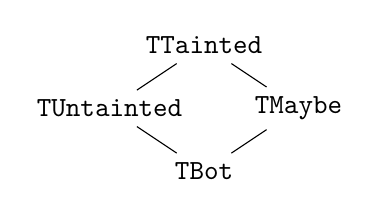
\begin{tikzpicture}[scale=0.8]
  \node (top) at (0,2) {\texttt{TTainted}};
  \node (untainted) at (-1.5,1) {\texttt{TUntainted}};
  \node (maybe) at (1.5,1) {\texttt{TMaybe}};
  \node (bot) at (0,0) {\texttt{TBot}};
  \draw (bot) -- (untainted) -- (top);
  \draw (bot) -- (maybe) -- (top);
\end{tikzpicture}
\end{center}
\textbf{Critical insight:} The \texttt{TMaybe} element breaks the Galois insertion property.
This means taint analysis can prove the \emph{presence} of bugs (true positives) but
\emph{cannot} prove their absence. See the code comments for detailed explanation.
\end{definition}

\begin{fstarcode}[title=Taint Domain - For Information Flow Analysis]
(* TAINT DOMAIN
   Source: Denning 1977 (information flow), Livshits 2005 (taint tracking)
   Used for: SQL injection, XSS, command injection, path traversal

   KEY INSIGHT: Taint analysis is a security analysis that tracks
   "trust level" of data through the program. Data from untrusted
   sources (user input) is TTainted; data from trusted sources is TUntainted.
   A bug exists when TTainted data reaches a sensitive sink. *)

type taint_level =
  | TBot        (* Unreachable *)
  | TUntainted  (* Known safe - from trusted sources *)
  | TMaybe      (* Unknown - could be either *)
  | TTainted    (* Definitely tainted - from untrusted sources *)

(* Taint forms a diamond lattice:
              TTainted
              /      \
        TUntainted   TMaybe
              \      /
               TBot
*)

let taint_leq (t1 t2 : taint_level) : bool =
  match t1, t2 with
  | TBot, _ -> true
  | _, TTainted -> true
  | TUntainted, TUntainted -> true
  | TUntainted, TMaybe -> true
  | TMaybe, TMaybe -> true
  | _, _ -> false

let taint_join (t1 t2 : taint_level) : taint_level =
  match t1, t2 with
  | TBot, t | t, TBot -> t
  | TTainted, _ | _, TTainted -> TTainted
  | TUntainted, TUntainted -> TUntainted
  | _, _ -> TMaybe

let taint_meet (t1 t2 : taint_level) : taint_level =
  match t1, t2 with
  | TTainted, t | t, TTainted -> t
  | TBot, _ | _, TBot -> TBot
  | TUntainted, TUntainted -> TUntainted
  | _, _ -> TUntainted  (* Conservative: meet with unknown is safe *)

instance taint_domain : abstract_domain taint_level = {
  lat = {
    po = { leq = taint_leq; (* ... *) };
    bot = TBot;
    top = TTainted;
    join = taint_join;
    meet = taint_meet;
    (* ... *)
  };
  widen = None;  (* Finite domain, no widening needed *)
  narrow = None;
}

(* IMPORTANT: TMaybe BREAKS GALOIS INSERTION
   The taint lattice with TMaybe does NOT form a Galois insertion because:
   - gamma(TMaybe) = "all concrete states" (we don't know)
   - alpha(gamma(TMaybe)) = TTainted (abstracting "all" gives tainted)
   - But TMaybe != TTainted, so alpha . gamma != id

   CONSEQUENCE: Taint analysis can only prove INCORRECTNESS (bugs exist),
   not correctness (no bugs). This aligns with the dual soundness principle
   (Section 2.1.8): use over-approximation for safety, under-approximation
   for bug-finding. Taint findings are REAL bugs, not false positives,
   but absence of findings does NOT guarantee safety. *)

(* Taint propagation: any tainted input taints output *)
let taint_propagate (inputs : list taint_level) : taint_level =
  List.fold_left taint_join TBot inputs
\end{fstarcode}

\begin{fstarcode}[title=Nullability Domain - For Null Pointer Analysis]
(* NULLABILITY DOMAIN
   Used for: Null dereference, optional value tracking, uninitialized vars *)

type nullability =
  | NBot       (* Unreachable *)
  | NNull      (* Definitely null *)
  | NNonNull   (* Definitely not null *)
  | NMaybe     (* Could be either - TOP *)

let nullability_leq (n1 n2 : nullability) : bool =
  match n1, n2 with
  | NBot, _ -> true
  | _, NMaybe -> true
  | NNull, NNull -> true
  | NNonNull, NNonNull -> true
  | _, _ -> false

let nullability_join (n1 n2 : nullability) : nullability =
  match n1, n2 with
  | NBot, n | n, NBot -> n
  | NNull, NNull -> NNull
  | NNonNull, NNonNull -> NNonNull
  | _, _ -> NMaybe

instance nullability_domain : abstract_domain nullability = {
  lat = {
    bot = NBot;
    top = NMaybe;
    join = nullability_join;
    meet = nullability_meet;
    (* ... *)
  };
  widen = None;
  narrow = None;
}

(* After null check: refine nullability *)
let after_null_check (n : nullability) (is_null_branch : bool) : nullability =
  match n, is_null_branch with
  | NMaybe, true -> NNull      (* In "if x == null" branch, x is null *)
  | NMaybe, false -> NNonNull  (* In "if x != null" branch, x is non-null *)
  | _, _ -> n
\end{fstarcode}

\begin{fstarcode}[title=Resource State Domain - For Lifecycle Analysis]
(* RESOURCE STATE DOMAIN
   Source: theory.md Chapter 14
   Used for: Use-after-free, double-free, resource leaks, file handles *)

type resource_state =
  | RSBot         (* Unreachable *)
  | RSUnacquired  (* Not yet acquired *)
  | RSAcquired    (* Acquired, ready for use *)
  | RSInUse       (* Currently being used *)
  | RSReleased    (* Released, cannot be used *)
  | RSTop         (* Unknown state *)

(* State machine transitions:
    Unacquired --acquire--> Acquired --use--> InUse
                               |                |
                               |                |
                               v                v
                           Released <--release--+

   Violations:
   - RSReleased -> use = UseAfterFree
   - RSReleased -> release = DoubleFree
   - RSAcquired at scope exit = Leak *)

let resource_leq (r1 r2 : resource_state) : bool =
  match r1, r2 with
  | RSBot, _ -> true
  | _, RSTop -> true
  | RSUnacquired, RSUnacquired -> true
  | RSAcquired, RSAcquired -> true
  | RSInUse, RSInUse -> true
  | RSReleased, RSReleased -> true
  | _, _ -> false

let resource_join (r1 r2 : resource_state) : resource_state =
  match r1, r2 with
  | RSBot, r | r, RSBot -> r
  | RSTop, _ | _, RSTop -> RSTop
  | r1, r2 when r1 = r2 -> r1
  | _, _ -> RSTop  (* Different states merge to unknown *)

(* Transfer functions for resource operations *)
let resource_acquire (r : resource_state) : resource_state * option resource_error =
  match r with
  | RSBot -> (RSBot, None)
  | RSUnacquired -> (RSAcquired, None)
  | RSAcquired -> (RSTop, Some DoubleAcquire)
  | RSInUse -> (RSTop, Some DoubleAcquire)
  | RSReleased -> (RSAcquired, None)  (* Re-acquire after release is OK *)
  | RSTop -> (RSTop, None)

let resource_use (r : resource_state) : resource_state * option resource_error =
  match r with
  | RSBot -> (RSBot, None)
  | RSUnacquired -> (RSTop, Some UseBeforeAcquire)
  | RSAcquired -> (RSInUse, None)
  | RSInUse -> (RSInUse, None)
  | RSReleased -> (RSTop, Some UseAfterRelease)
  | RSTop -> (RSTop, None)

let resource_release (r : resource_state) : resource_state * option resource_error =
  match r with
  | RSBot -> (RSBot, None)
  | RSUnacquired -> (RSTop, Some ReleaseBeforeAcquire)
  | RSAcquired -> (RSReleased, None)
  | RSInUse -> (RSReleased, None)
  | RSReleased -> (RSTop, Some DoubleRelease)
  | RSTop -> (RSTop, None)

type resource_error =
  | UseBeforeAcquire
  | UseAfterRelease
  | DoubleAcquire
  | DoubleRelease
  | ReleaseBeforeAcquire
  | LeakOnExit

instance resource_domain : abstract_domain resource_state = {
  lat = { bot = RSBot; top = RSTop; join = resource_join; (* ... *) };
  widen = None;
  narrow = None;
}
\end{fstarcode}

\begin{fstarcode}[title=Ownership Domain - For Memory Safety Analysis]
(* OWNERSHIP DOMAIN
   Source: Girard 1987 (substructural logic), Jung 2018 (Iris/RustBelt)
   Used for: Ownership tracking (Rust-style AFFINE), borrow checking, move detection

   NOTE: Rust uses AFFINE typing (use at most once, can drop without use).
   Strictly LINEAR requires exactly one use. We model the affine fragment. *)

type ownership =
  | OBot         (* Unreachable *)
  | OUnowned     (* Not owned by anyone *)
  | OOwned       (* Exclusively owned *)
  | OBorrowed    (* Temporarily borrowed (immutable) *)
  | OMutBorrowed (* Temporarily borrowed (mutable) *)
  | OShared      (* Reference-counted / shared *)
  | OMoved       (* Ownership transferred away *)
  | OTop         (* Unknown *)

(* Ownership rules (from RustBelt):
   - Owned can be moved or borrowed
   - Borrowed can be cloned (shared borrow)
   - MutBorrowed is exclusive
   - Moved cannot be used *)

let ownership_leq (o1 o2 : ownership) : bool =
  match o1, o2 with
  | OBot, _ -> true
  | _, OTop -> true
  | o1, o2 when o1 = o2 -> true
  | _, _ -> false

let ownership_join (o1 o2 : ownership) : ownership =
  match o1, o2 with
  | OBot, o | o, OBot -> o
  | OTop, _ | _, OTop -> OTop
  | o1, o2 when o1 = o2 -> o1
  | OOwned, OBorrowed | OBorrowed, OOwned -> OOwned  (* Borrow ends *)
  | _, _ -> OTop

(* Transfer functions *)
let ownership_move (o : ownership) : ownership * option ownership_error =
  match o with
  | OOwned -> (OMoved, None)
  | OMoved -> (OTop, Some UseAfterMove)
  | OBorrowed -> (OTop, Some MoveWhileBorrowed)
  | OMutBorrowed -> (OTop, Some MoveWhileBorrowed)
  | _ -> (OTop, None)

let ownership_borrow (o : ownership) : ownership * option ownership_error =
  match o with
  | OOwned -> (OBorrowed, None)
  | OBorrowed -> (OBorrowed, None)  (* Can borrow from borrow *)
  | OMutBorrowed -> (OTop, Some BorrowWhileMutBorrowed)
  | OMoved -> (OTop, Some UseAfterMove)
  | _ -> (OTop, None)

let ownership_mut_borrow (o : ownership) : ownership * option ownership_error =
  match o with
  | OOwned -> (OMutBorrowed, None)
  | OBorrowed -> (OTop, Some MutBorrowWhileBorrowed)
  | OMutBorrowed -> (OTop, Some MutBorrowWhileMutBorrowed)
  | OMoved -> (OTop, Some UseAfterMove)
  | _ -> (OTop, None)

type ownership_error =
  | UseAfterMove
  | MoveWhileBorrowed
  | BorrowWhileMutBorrowed
  | MutBorrowWhileBorrowed
  | MutBorrowWhileMutBorrowed
\end{fstarcode}

%--------------------------------------------------
\section{Occurrence Type Domain}
%--------------------------------------------------

\noindent\textbf{Source:} Tobin-Hochstadt \& Felleisen 2008 (Typed Scheme)

\begin{tcolorbox}[
  title={\textbf{Occurrence Typing: Flow-Sensitive Type Refinement via Predicates}},
  colback=blue!5,
  colframe=blue!70!black,
  fonttitle=\bfseries,
  breakable
]
\textbf{Problem:} Union types lose precision after type tests.
\begin{lstlisting}[language=Python,basicstyle=\small\ttfamily]
def process(x: int | str) -> int:
  if isinstance(x, str):
    return len(x)    # Type of x should be str here, not int|str!
  return x           # Type of x should be int here
\end{lstlisting}

\textbf{Solution:} Track TYPE PROPOSITIONS through control flow.
\begin{itemize}
  \item Type tests generate predicates about variables
  \item Branch conditions refine types in each branch
  \item Join points combine refinements conservatively
\end{itemize}

\textbf{Complements Gradual Typing (Section 9.1.2):}
\begin{itemize}
  \item Gradual typing: \texttt{?} type at module BOUNDARIES
  \item Occurrence typing: Refinement WITHIN module from type tests
  \item Together: Sound dynamic + static typing in same codebase
\end{itemize}
\end{tcolorbox}

\begin{definition}[Key Concepts from Tobin-Hochstadt 2008]
\textbf{Visible vs Latent Predicates:}
\begin{itemize}
  \item \textbf{Visible:} Type proposition known to hold at current point.\\
    Example: After \texttt{if isinstance(x, str):} we have visible predicate $x:\mathsf{str}$
  \item \textbf{Latent:} Type proposition attached to a function result.\\
    Example: \texttt{string?(v)} returns true implies $v$ has type $\mathsf{str}$.
    The function ``remembers'' what type test it performed.
\end{itemize}

\textbf{Propositional Type Environments (Section 3.2):}
\begin{align*}
  \Gamma &= \{x : \tau, \ldots\} \quad \text{(Standard type assignment)} \\
  \Gamma|\psi &= \text{Environment refined by proposition } \psi \\
  \psi &::= \tau(x) \mid \lnot\tau(x) \mid \psi_1 \land \psi_2 \mid \psi_1 \lor \psi_2 \mid \mathsf{true} \mid \mathsf{false}
\end{align*}

\textbf{Environment Refinement Operations:}
\begin{align*}
  \Gamma + \psi &= \text{Environment assuming } \psi \text{ is TRUE} \\
  \Gamma + \tau(x) &= \Gamma[x := \Gamma(x) \cap \tau] \quad \text{(Restrict } x \text{ to } \tau\text{)} \\
  \Gamma + \lnot\tau(x) &= \Gamma[x := \Gamma(x) - \tau] \quad \text{(Remove } \tau \text{ from } x\text{)} \\
  \Gamma - \psi &= \Gamma + \lnot\psi \quad \text{(Environment assuming } \psi \text{ is FALSE)}
\end{align*}

\textbf{Type Operations:}
\begin{align*}
  \mathsf{restrict}(\sigma, \tau) &= \sigma \cap \tau \quad \text{(Narrow } \sigma \text{ to } \tau\text{)} \\
  \mathsf{remove}(\sigma, \tau) &= \sigma - \tau \quad \text{(Remove } \tau \text{ from } \sigma\text{)}
\end{align*}
\end{definition}

\begin{fstarcode}[title=Occurrence Type Domain (Tobin-Hochstadt \& Felleisen 2008)]
module BrrrMachine.Domains.Occurrence

(* TYPE PROPOSITIONS
   Propositions express facts about the types of variables. *)
type type_prop =
  | PropHasType : var:string -> ty:ir_type -> type_prop
      (* var has type ty *)
  | PropNotType : var:string -> ty:ir_type -> type_prop
      (* var does NOT have type ty *)
  | PropAnd : type_prop -> type_prop -> type_prop
  | PropOr : type_prop -> type_prop -> type_prop
  | PropTrue : type_prop
  | PropFalse : type_prop  (* Contradiction - unreachable *)

(* Negate a proposition *)
let rec negate_prop (p : type_prop) : type_prop =
  match p with
  | PropHasType v t -> PropNotType v t
  | PropNotType v t -> PropHasType v t
  | PropAnd p1 p2 -> PropOr (negate_prop p1) (negate_prop p2)
  | PropOr p1 p2 -> PropAnd (negate_prop p1) (negate_prop p2)
  | PropTrue -> PropFalse
  | PropFalse -> PropTrue

(* VISIBLE AND LATENT PREDICATES *)
type visible_predicate = {
  prop : type_prop;
  source : node_id;        (* Where predicate was established *)
}

type latent_predicate = {
  positive : type_prop;    (* Proposition if function returns true *)
  negative : type_prop;    (* Proposition if function returns false *)
  target_var : option string; (* Variable the predicate applies to *)
}

(* Type predicates built into languages *)
let builtin_predicates : map string latent_predicate = Map.of_list [
  (* Python *)
  ("isinstance", { positive = PropTrue; negative = PropTrue; target_var = None });
  (* TypeScript *)
  ("typeof", { positive = PropTrue; negative = PropTrue; target_var = None });
  (* Go *)
  ("type_assertion", { positive = PropTrue; negative = PropTrue; target_var = None });
]

(* TYPE RESTRICTION AND REMOVAL *)
(* restrict(sigma, tau) = sigma intersect tau *)
let rec restrict (sigma : ir_type) (tau : ir_type) : ir_type =
  match sigma with
  | TUnion types ->
      let restricted = List.filter_map (fun t ->
        let r = restrict t tau in
        if is_bottom r then None else Some r
      ) types in
      (match restricted with
       | [] -> TBottom
       | [t] -> t
       | ts -> TUnion ts)
  | _ ->
      if subtype sigma tau then sigma
      else if subtype tau sigma then tau
      else TBottom

(* remove(sigma, tau) = sigma minus tau *)
let rec remove (sigma : ir_type) (tau : ir_type) : ir_type =
  match sigma with
  | TUnion types ->
      let remaining = List.filter_map (fun t ->
        let r = remove t tau in
        if is_bottom r then None else Some r
      ) types in
      (match remaining with
       | [] -> TBottom
       | [t] -> t
       | ts -> TUnion ts)
  | _ ->
      if subtype sigma tau then TBottom
      else sigma
\end{fstarcode}

\begin{fstarcode}[title=Propositional Type Environment]
(* Maps variables to types, refined by propositions. *)
type prop_type_env = {
  bindings : map string ir_type;
  active_props : list visible_predicate;
}

(* Refine environment assuming proposition is TRUE: Gamma + psi *)
let rec refine_positive (env : prop_type_env) (prop : type_prop) : prop_type_env =
  match prop with
  | PropHasType var ty ->
      (match Map.find var env.bindings with
       | Some current_ty ->
           let refined = restrict current_ty ty in
           { env with bindings = Map.add var refined env.bindings }
       | None -> env)
  | PropNotType var ty ->
      (match Map.find var env.bindings with
       | Some current_ty ->
           let refined = remove current_ty ty in
           { env with bindings = Map.add var refined env.bindings }
       | None -> env)
  | PropAnd p1 p2 ->
      refine_positive (refine_positive env p1) p2
  | PropOr p1 p2 ->
      (* Conservative: only refine if BOTH branches agree *)
      let env1 = refine_positive env p1 in
      let env2 = refine_positive env p2 in
      join_environments env1 env2
  | PropTrue -> env
  | PropFalse ->
      (* Unreachable - mark all types as bottom *)
      { env with bindings = Map.map (fun _ -> TBottom) env.bindings }

(* Refine environment assuming proposition is FALSE: Gamma - psi *)
let refine_negative (env : prop_type_env) (prop : type_prop) : prop_type_env =
  refine_positive env (negate_prop prop)

(* Join two environments at control flow merge *)
let join_environments (env1 env2 : prop_type_env) : prop_type_env =
  let bindings = Map.merge (fun _ t1 t2 ->
    match t1, t2 with
    | Some t1, Some t2 -> Some (type_join t1 t2)
    | Some t, None | None, Some t -> Some t
    | None, None -> None
  ) env1.bindings env2.bindings in
  { bindings; active_props = [] }  (* Props lost at join *)
\end{fstarcode}

\begin{fstarcode}[title=Type Predicate Detection]
(* Detect type-testing patterns in code. *)
type type_test_result = {
  tested_var : string;
  test_type : ir_type;
  is_positive : bool;       (* true = "is type", false = "is not type" *)
}

(* Detect isinstance(x, T) pattern in Python *)
let detect_isinstance (call : ir_expr) : option type_test_result =
  match call with
  | ECall (EVar "isinstance") [EVar var; EType ty] ->
      Some { tested_var = var; test_type = ty; is_positive = true }
  | _ -> None

(* Detect typeof x === "T" pattern in TypeScript/JavaScript *)
let detect_typeof (expr : ir_expr) : option type_test_result =
  match expr with
  | EBinOp OpEq (ECall (EVar "typeof") [EVar var]) (EString ty_name) ->
      let ty = string_to_type ty_name in
      Some { tested_var = var; test_type = ty; is_positive = true }
  | EBinOp OpNeq (ECall (EVar "typeof") [EVar var]) (EString ty_name) ->
      let ty = string_to_type ty_name in
      Some { tested_var = var; test_type = ty; is_positive = false }
  | _ -> None

(* Detect x !== null / x !== undefined pattern *)
let detect_null_check (expr : ir_expr) : option type_test_result =
  match expr with
  | EBinOp OpNeq (EVar var) ENull ->
      Some { tested_var = var; test_type = TNull; is_positive = false }
  | EBinOp OpNeq (EVar var) EUndefined ->
      Some { tested_var = var; test_type = TUndefined; is_positive = false }
  | EBinOp OpEq (EVar var) ENull ->
      Some { tested_var = var; test_type = TNull; is_positive = true }
  | _ -> None

(* Detect "key" in obj pattern for TypeScript discriminated unions *)
let detect_in_check (expr : ir_expr) : option type_test_result =
  match expr with
  | EBinOp OpIn (EString key) (EVar var) ->
      (* Having key means var has type with that property *)
      Some { tested_var = var;
             test_type = TWithProperty key;
             is_positive = true }
  | _ -> None
\end{fstarcode}

\begin{fstarcode}[title=Occurrence Typing Transfer Function and Lattice]
(* OCCURRENCE TYPING TRANSFER FUNCTION *)
val occurrence_transfer : prop_type_env -> ir_stmt -> prop_type_env

let occurrence_transfer env stmt =
  match stmt with
  | SIf cond then_branch else_branch ->
      (* Detect type test in condition *)
      let test = detect_type_test cond in
      (match test with
       | Some { tested_var; test_type; is_positive } ->
           let true_prop =
             if is_positive then PropHasType tested_var test_type
             else PropNotType tested_var test_type in
           (* Refine environments for each branch *)
           let then_env = refine_positive env true_prop in
           let else_env = refine_negative env true_prop in
           (* Join at merge point *)
           join_environments then_env else_env
       | None -> env)
  | SAssign var expr ->
      (* Assignment overwrites type - no longer refined *)
      { env with
        bindings = Map.add var (infer_type expr) env.bindings;
        active_props = List.filter (fun p ->
          not (prop_mentions_var p.prop var)
        ) env.active_props }
  | _ -> env

(* INTEGRATION WITH ABSTRACT INTERPRETATION *)
type occurrence_domain = {
  env : prop_type_env;
}

let occurrence_lattice : lattice occurrence_domain = {
  bot = { env = { bindings = Map.empty; active_props = [] } };
  top = { env = { bindings = Map.singleton "_" TTop; active_props = [] } };
  leq = fun d1 d2 ->
    Map.for_all (fun v t1 ->
      match Map.find v d2.env.bindings with
      | Some t2 -> subtype t1 t2
      | None -> true
    ) d1.env.bindings;
  join = fun d1 d2 ->
    { env = join_environments d1.env d2.env };
  meet = fun d1 d2 ->
    { env = {
        bindings = Map.merge (fun _ t1 t2 ->
          match t1, t2 with
          | Some t1, Some t2 -> Some (type_meet t1 t2)
          | _ -> None
        ) d1.env.bindings d2.env.bindings;
        active_props = d1.env.active_props @ d2.env.active_props
      } };
}
\end{fstarcode}

\textbf{Cross-References:}
\begin{itemize}
  \item Section 9.1.2: Occurrence typing complements gradual typing at boundaries
  \item Section 9.3: Guards can use occurrence typing propositions
  \item Section 9.5: Full occurrence typing analysis algorithm
  \item Section 12.3.5: F* soundness theorem for occurrence typing
\end{itemize}

%--------------------------------------------------
\section{DeepPoly: Abstract Domain for Neural Networks}
%--------------------------------------------------

\noindent\textbf{Paper:} Singh, Gehr, Puschel, Vechev 2019 (POPL)

\begin{tcolorbox}[
  title={\textbf{Neural Network Verification via Abstract Interpretation}},
  colback=green!5,
  colframe=green!70!black,
  fonttitle=\bfseries,
  breakable
]
\textbf{Problem:} Neural networks in safety-critical systems (autonomous driving, medical diagnosis) require robustness certification. Prior methods (SMT, MILP) cannot scale beyond $\sim$2K neurons.

\textbf{DeepPoly Insight:} Restricted polyhedral domain with backsubstitution.
\begin{itemize}
  \item One lower bound + one upper bound per neuron (prevents blowup)
  \item Affine expressions relate neurons to predecessors
  \item Backsubstitution computes tight bounds through layers
\end{itemize}

\textbf{Abstract Element} for neuron $x_i$:
\[
  a_i = (a_i^{\leq}, a_i^{\geq}, l_i, u_i)
\]
where:
\begin{align*}
  a_i^{\leq}(x) \leq x_i \leq a_i^{\geq}(x) &\quad \text{(symbolic polyhedral bounds)} \\
  l_i \leq x_i \leq u_i &\quad \text{(concrete interval bounds)}
\end{align*}

\textbf{Key Transformers:}
\begin{itemize}
  \item Affine layer: EXACT (no precision loss)
  \item ReLU layer: Area-minimizing linear approximation (sound)
  \item Sigmoid/Tanh: Tangent-based linear bounds (sound)
\end{itemize}

\textbf{Performance:} 100--1000x faster than MILP, scales to 62K neurons.
\end{tcolorbox}

\begin{remark}[ReLU Approximation Strategy]
For $\mathsf{ReLU}(x) = \max(0, x)$ when interval crosses zero ($l < 0 < u$):

Two candidate approximations based on AREA MINIMIZATION:
\begin{itemize}
  \item Option (b): Lower = 0, Upper = $\lambda x + \mu$ (area = $0.5 \cdot u \cdot (u-l)$)
  \item Option (c): Lower = $x$, Upper = $\lambda x + \mu$ (area = $0.5 \cdot (-l) \cdot (u-l)$)
\end{itemize}
Choose the option with SMALLER area in $(x, \text{output})$ plane. This geometric insight is KEY to DeepPoly's precision.
\end{remark}

\begin{remark}[Backsubstitution for Precision]
To compute tight bounds for neuron $x_i$:
\begin{enumerate}
  \item Start with symbolic constraint $a_i(x_0, \ldots, x_{i-1})$
  \item Recursively substitute constraints for intermediate neurons
  \item Continue until only INPUT variables remain
  \item Apply concrete input bounds to get tight interval
\end{enumerate}
This enables RELATIONAL reasoning across many layers without storing exponential constraints.
\end{remark}

The following F* code implements the DeepPoly abstract domain. The key type is
\texttt{neuron\_constraint}, which stores both symbolic polyhedral bounds (affine expressions
relating to predecessors) and concrete interval bounds. The \texttt{relu\_transform} function
implements the area-minimizing approximation for ReLU neurons.

\begin{fstarcode}[title=DeepPoly Abstract Domain for Neural Networks (Singh et al.\ POPL 2019)]
(* This module implements the DeepPoly abstract domain for neural network
   verification. The key insight is to maintain RELATIONAL constraints between
   neurons (via affine expressions) while using backsubstitution to compute
   tight bounds. This achieves much better precision than interval analysis
   while remaining tractable for large networks. *)

module BrrrMachine.Domains.DeepPoly

(* Affine expression: c_0 + sum(c_i * x_i) *)
type affine_expr = {
  const : real;
  coeffs : list (nat * real);  (* (neuron_index, coefficient) *)
}

(* DeepPoly constraint for single neuron *)
type neuron_constraint = {
  nc_lower : affine_expr;     (* Lower polyhedral bound *)
  nc_upper : affine_expr;     (* Upper polyhedral bound *)
  nc_lo : real;               (* Interval lower bound *)
  nc_hi : real;               (* Interval upper bound *)
}

(* Network abstract state *)
type deeppoly_state = {
  constraints : list neuron_constraint;
  input_bounds : list (real * real);
  num_inputs : nat;
}

(* Concretization: set of all concrete values satisfying constraints *)
val gamma : deeppoly_state -> set (list real)

(* RELU TRANSFORMER - Area-minimizing approximation *)
val relu_transform : neuron_constraint -> neuron_constraint
let relu_transform nc =
  if nc.nc_hi <= 0.0 then
    (* Always inactive: output = 0 *)
    { nc_lower = { const = 0.0; coeffs = [] };
      nc_upper = { const = 0.0; coeffs = [] };
      nc_lo = 0.0; nc_hi = 0.0 }
  else if nc.nc_lo >= 0.0 then
    (* Always active: identity *)
    nc
  else
    (* Crossing zero: area-minimizing approximation *)
    let lambda = nc.nc_hi /. (nc.nc_hi -. nc.nc_lo) in
    let mu = -. nc.nc_lo *. nc.nc_hi /. (nc.nc_hi -. nc.nc_lo) in
    (* Choose smaller area: compare |u| vs |l| *)
    if nc.nc_hi <= -. nc.nc_lo then
      (* Option (b): lower = 0 has smaller area *)
      { nc_lower = { const = 0.0; coeffs = [] };
        nc_upper = scale_add_affine lambda nc.nc_upper mu;
        nc_lo = 0.0; nc_hi = nc.nc_hi }
    else
      (* Option (c): lower = x has smaller area *)
      { nc_lower = nc.nc_lower;
        nc_upper = scale_add_affine lambda nc.nc_upper mu;
        nc_lo = nc.nc_lo; nc_hi = nc.nc_hi }

(* BACKSUBSTITUTION - Compute tight bounds via recursive substitution *)
val backsubstitute :
  constraints:list neuron_constraint ->
  expr:affine_expr ->
  input_bounds:list (real * real) ->
  (real * real)  (* Tight lower and upper bounds *)

(* SOUNDNESS THEOREMS *)
val affine_layer_exact :
  state:deeppoly_state -> weights:matrix -> bias:list real ->
  Lemma (gamma (transform_affine state weights bias) =
         image (apply_affine weights bias) (gamma state))

val relu_layer_sound :
  state:deeppoly_state ->
  Lemma (image apply_relu (gamma state) `subset`
         gamma (transform_relu state))

val network_certification_sound :
  layers:list layer -> input_region:deeppoly_state ->
  Lemma (forall x. x `in` gamma input_region ==>
         network_output layers x `in` gamma (analyze layers input_region))
\end{fstarcode}

\begin{remark}[Domain Taxonomy Extension]
DeepPoly introduces a new category of abstract domains:

\textbf{Domain Precision Hierarchy (extended):}
\[
  \text{Intervals} < \text{Zonotopes} < \text{DeepPoly} < \text{Full Polyhedra} < \text{MILP}
\]
\hfill (fast) \hspace{8cm} (slow)

DeepPoly achieves a sweet spot:
\begin{itemize}
  \item More precise than intervals/zonotopes (relational constraints)
  \item Much faster than polyhedra/MILP (restricted form)
  \item Scales to production networks (62K+ neurons)
\end{itemize}
\end{remark}

\textbf{Cross-References:}
\begin{itemize}
  \item Section 2.1.6: Abstract domain formalization (DeepPoly is an instance)
  \item Section 2.1.7: Concrete domains (DeepPoly extends this taxonomy)
  \item Section 2.1.5c: Neural invariant synthesis (complementary technique)
\end{itemize}

%--------------------------------------------------
\section{Dual Soundness: Over and Under Approximation}
%--------------------------------------------------

\noindent\textbf{Papers:} O'Hearn 2020 (Incorrectness Logic - historical, superseded by OL), Zilberstein 2023 (Outcome Logic)

\begin{tcolorbox}[
  title={\textbf{Critical Insight: Analysis Soundness Has Two Dual Forms}},
  colback=red!5,
  colframe=red!70!black,
  fonttitle=\bfseries,
  breakable
]
The synthesis previously conflated these --- they serve DIFFERENT purposes.
\end{tcolorbox}

\begin{definition}[Verification Soundness (Over-Approximation)]
\[
  \alpha(\text{concrete}) \subseteq \text{abstract}
\]
``If analysis says SAFE, it truly is safe.''
\begin{itemize}
  \item May have FALSE POSITIVES (false alarms)
  \item Cannot have false negatives (missed bugs)
  \item Used for: proving absence of bugs, verification
\end{itemize}
This is what Cousot abstract interpretation provides.
\end{definition}

\begin{definition}[Detection Soundness (Under-Approximation)]
\[
  \text{abstract} \subseteq \text{concrete}
\]
``If analysis says BUG, it truly is a bug.''
\begin{itemize}
  \item May have FALSE NEGATIVES (missed bugs)
  \item Cannot have false positives (false alarms)
  \item Used for: proving presence of bugs, bug finding
\end{itemize}
This is what O'Hearn's Incorrectness Logic provided historically, now superseded by Outcome Logic (OL).
\end{definition}

\begin{tcolorbox}[
  title={\textbf{The Brrr-Machine Needs Both}},
  colback=gray!5,
  colframe=gray!60,
  breakable
]
\begin{center}
\begin{tabular}{@{}ccc@{}}
\toprule
\textbf{Proven Safe} & \textbf{Uncertain} & \textbf{Proven Buggy} \\
(over-approx) & & (under-approx) \\
\midrule
No bugs exist & May have bugs & Bug definitely exists \\
100\% confident & Needs review & 100\% confident \\
\bottomrule
\end{tabular}
\end{center}
\end{tcolorbox}

\begin{remark}[Why This Matters]
\begin{enumerate}
  \item \textbf{Verification mode:} We want to PROVE code is safe. Use over-approximation. False positives acceptable; false negatives catastrophic.
  \item \textbf{Bug-finding mode:} We want to FIND real bugs. Use under-approximation. False negatives acceptable; false positives waste developer time.
  \item \textbf{Combined mode:} Use BOTH to classify findings into proven-safe, proven-buggy, and uncertain categories.
\end{enumerate}
\end{remark}

\begin{definition}[Consequence Rule Reversal]
\textbf{Hoare (over-approx):}
\begin{mathpar}
  \inferrule{p' \Rightarrow p \\ \{p\} C \{q\} \\ q \Rightarrow q'}
            {\{p'\} C \{q'\}}
\end{mathpar}
STRONGER pre, WEAKER post

\textbf{Incorrectness (under-approx):}
\begin{mathpar}
  \inferrule{p' \Leftarrow p \\ [p] C [q] \\ q' \Leftarrow q}
            {[p'] C [q']}
\end{mathpar}
WEAKER pre, STRONGER post
\end{definition}

\begin{definition}[Disjunction Behavior]
\textbf{Over-approx:} Must track ALL paths
\begin{mathpar}
  \inferrule{\{p_1\}C\{q_1\} \\ \{p_2\}C\{q_2\}}
            {\{p_1 \land p_2\}C\{q_1 \land q_2\}}
\end{mathpar}
Intersection of posts (must hold in both)

\textbf{Under-approx:} Can DROP paths
\begin{mathpar}
  \inferrule{[p_1]C[q_1] \\ [p_2]C[q_2]}
            {[p_1 \lor p_2]C[q_1 \lor q_2]}
\end{mathpar}
Union of posts (may drop one path!)

This justifies PARTIAL COVERAGE in bug-finding --- sound to forget paths.
\end{definition}

\begin{remark}[Integration with Outcome Logic (OL)]
\textbf{Critical:} Incorrectness Logic (IL) is incompatible with abstract interpretation (Ascari et al.\ 2022). OL fixes this while preserving IL's true-positive property.

\textbf{Why OL Over IL:}
\begin{enumerate}
  \item IL breaks abstraction --- reverse consequence rule + abstract AI don't compose
  \item IL's ``One-Sided If'' generates imprecise preconditions
  \item IL can't handle probabilistic programs
\end{enumerate}

\textbf{OL provides:}
\begin{itemize}
  \item Unified framework for correctness AND incorrectness
  \item Compatible with abstract interpretation
  \item Manifest/latent bug classification (see Section 12.5)
  \item Falsification completeness (Theorem 5.1)
\end{itemize}

Use OL as the foundation for dual-mode analysis.
\end{remark}

See Section 12.4 for formal theorems and Section 12.5 for manifest error detection.

%--------------------------------------------------
\section{Local Completeness Logic (Bruni et al.\ 2023)}
%--------------------------------------------------

\noindent\textbf{Paper:} Bruni, Giacobazzi, Gori, Ranzato 2023 (A Correctness and Incorrectness Program Logic)

\begin{tcolorbox}[
  title={\textbf{Key Insight: Local Completeness Bridges Over/Under Approximation}},
  colback=blue!5,
  colframe=blue!70!black,
  fonttitle=\bfseries,
  breakable
]
Global completeness ($\alpha \circ f = f^\sharp \circ \alpha$) is RARE --- only trivial domains achieve it.

LOCAL completeness (at specific inputs) is ACHIEVABLE and USEFUL.

$\mathsf{LCL}_A$ combines BOTH correctness AND incorrectness in ONE framework, parameterized by abstract domain $A$.
\end{tcolorbox}

\begin{theorem}[Global Completeness Is Rare (Giacobazzi et al.\ 2015, Theorem 4.5)]
For Turing-complete languages, only TRIVIAL domains are globally complete:
\begin{enumerate}
  \item Identity abstraction (concrete = abstract) --- useless
  \item Top abstraction (all programs equivalent) --- useless
\end{enumerate}

\textbf{Consequence:} For any useful abstract domain, there exist inputs where the analysis produces false alarms (over-approximation is imprecise).

\textbf{The Solution:} LOCAL COMPLETENESS --- Instead of requiring completeness for ALL inputs, require it only for SPECIFIC inputs of interest.
\end{theorem}

\begin{definition}[Local Completeness (Definition 4.1)]
Abstract domain $A$ is \emph{locally complete} for $f:C \to C$ at concrete value $c \in C$, written $\mathcal{C}^A_c(f)$, if:
\[
  \mathcal{C}^A_c(f) \iff \alpha \circ f(c) = \alpha \circ f \circ \gamma \circ \alpha(c)
\]
Meaning: For input $c$, the abstraction of $f(c)$ equals the abstraction of applying $f$ to the ``best'' approximation of $c$.

\textbf{Global vs Local:}
\begin{align*}
  \text{Global:} & \quad \forall c \in C.\; \mathcal{C}^A_c(f) \quad \text{(for all inputs --- rare)} \\
  \text{Local:} & \quad \mathcal{C}^A_c(f) \quad \text{(for specific input } c \text{ --- achievable)}
\end{align*}
\end{definition}

\begin{definition}[The $\mathsf{LCL}_A$ Proof System]
\textbf{$\mathsf{LCL}_A$ Triple:} $\vdash_A [p]\, r\, [q]$

Meaning:
\begin{enumerate}
  \item $q \subseteq \sem{r}p$ \hfill ($q$ under-approximates strongest postcondition)
  \item $\mathcal{C}^A_p(r)$ holds \hfill ($r$ is locally complete for input $p$ in $A$)
  \item $\alpha(q) = \alpha(\sem{r}p)$ \hfill (abstractions coincide)
\end{enumerate}

\textbf{Key Insight:} If $\vdash_A [p]\, r\, [q]$ is provable, then:
\begin{itemize}
  \item $q$ contains only TRUE alarms (under-approximation property)
  \item If $q$ has no alarms, then $\sem{r}p$ has no alarms (completeness at $p$)
  \item The analysis is BOTH sound for bugs AND complete for safety at $p$
\end{itemize}
\end{definition}

\begin{definition}[Key Rules of $\mathsf{LCL}_A$]
\textbf{Transfer Rule:} Base case for primitive commands
\begin{mathpar}
  \inferrule{\mathcal{C}^A_p(e)}
            {\vdash_A [p]\, e\, [\sem{e}p]}
  \quad \text{(transfer)}
\end{mathpar}

\textbf{Relax Rule:} Weaken precondition, strengthen postcondition (within abstraction)
\begin{mathpar}
  \inferrule{p' \subseteq p \subseteq \gamma(\alpha(p')) \\ \vdash_A [p']\, r\, [q'] \\ q \subseteq q' \subseteq \gamma(\alpha(q))}
            {\vdash_A [p]\, r\, [q]}
  \quad \text{(relax)}
\end{mathpar}

\textbf{Sequence Rule:} Composition
\begin{mathpar}
  \inferrule{\vdash_A [p]\, r_1\, [w] \\ \vdash_A [w]\, r_2\, [q]}
            {\vdash_A [p]\, r_1;r_2\, [q]}
  \quad \text{(seq)}
\end{mathpar}

\textbf{Join Rule:} Non-deterministic choice
\begin{mathpar}
  \inferrule{\vdash_A [p]\, r_1\, [q_1] \\ \vdash_A [p]\, r_2\, [q_2]}
            {\vdash_A [p]\, r_1+r_2\, [q_1 \cup q_2]}
  \quad \text{(join)}
\end{mathpar}

\textbf{Iterate Rule:} Loop with local completeness check
\begin{mathpar}
  \inferrule{\vdash_A [p]\, r\, [q] \\ q \subseteq \gamma(\alpha(p))}
            {\vdash_A [p]\, r^*\, [p \cup q]}
  \quad \text{(iterate)}
\end{mathpar}
\end{definition}

\begin{theorem}[Connection to Incorrectness Logic (Section 6)]
$\mathsf{IL} = \mathsf{LCL}_{A_{\mathsf{tr}}}$

When $A = A_{\mathsf{tr}}$ (the trivial ``top'' abstraction that makes all properties equivalent):
\begin{itemize}
  \item Every transfer function is globally complete in $A_{\mathsf{tr}}$
  \item $\mathsf{LCL}_{A_{\mathsf{tr}}}$ coincides EXACTLY with O'Hearn's Incorrectness Logic
  \item This is because $A_{\mathsf{tr}}$ provides NO precision --- can't distinguish any states
\end{itemize}

\textbf{Implication:}
\begin{itemize}
  \item IL is a SPECIAL CASE of $\mathsf{LCL}_A$
  \item For any non-trivial $A$, $\mathsf{LCL}_A$ is MORE POWERFUL than IL
  \item $\mathsf{LCL}_A$ can prove CORRECTNESS (when $q$ has no alarms)
  \item IL can only prove INCORRECTNESS (existence of bugs)
\end{itemize}
\end{theorem}

\begin{theorem}[Soundness of $\mathsf{LCL}_A$ (Theorem 5.5)]
If $\vdash_A [p]\, r\, [q]$ then:
\begin{enumerate}
  \item $q \subseteq \sem{r}p$ \hfill (under-approximation)
  \item $\sem{r}^\sharp_A \alpha(p) = \alpha(q) = \alpha(\sem{r}p)$ \hfill (local completeness)
\end{enumerate}
\end{theorem}

\begin{corollary}[Precision (Corollary 5.6)]
If $\vdash_A [p]\, r\, [q]$ then for all $a \in A$:
\[
  \sem{r}p \subseteq \gamma(a) \iff q \subseteq \gamma(a)
\]
Meaning: $q$ and $\sem{r}p$ have the SAME abstract over-approximations.
\end{corollary}

\begin{tcolorbox}[
  title={\textbf{Unified Tri-State Analysis Using $\mathsf{LCL}_A$}},
  colback=gray!5,
  colframe=gray!60,
  breakable
]
Given abstract domain $A$ and input $p$, analyze program $C$:

Attempt to prove $\vdash_A [p]\, C\, [q]$

\begin{description}
  \item[Case 1:] $q$ contains alarm states\\
    $\Rightarrow$ \textbf{Proven Buggy} (under-approximation guarantees true bugs)
  \item[Case 2:] $q$ contains no alarm states AND proof succeeds\\
    $\Rightarrow$ \textbf{Proven Safe} (local completeness at $p$ means no false negatives)
  \item[Case 3:] Proof fails (local completeness obligation not met)\\
    $\Rightarrow$ \textbf{Uncertain} (need more precise domain or different input abstraction)
\end{description}
\end{tcolorbox}

\begin{remark}[Domain Refinement for Local Completeness (Section 8)]
When local completeness fails, REFINE the domain.

If $\mathcal{C}^A_p(f)$ fails, we can:
\begin{enumerate}
  \item Compute the BEST CORRECT APPROXIMATION (bca) for $f$ at $p$
  \item Extend $A$ to include this value
  \item Re-attempt the proof with refined domain
\end{enumerate}
This gives a DIRECTED refinement strategy --- refine only where needed, not globally. Much more practical than complete abstract refinement.
\end{remark}

\begin{remark}[Integration with Outcome Logic]
\textbf{$\mathsf{LCL}_A$ + OL Integration:}

Both frameworks address over/under approximation unification:
\begin{itemize}
  \item OL (Zilberstein 2023): Unified semantics for correctness and incorrectness
  \item $\mathsf{LCL}_A$ (Bruni 2023): Unified proof system parameterized by abstract domain
\end{itemize}

\textbf{Recommended Approach:}
\begin{enumerate}
  \item Use OL for SEMANTICS (what correctness/incorrectness mean)
  \item Use $\mathsf{LCL}_A$ for ANALYSIS (how to compute verdicts)
  \item Abstract domain $A$ determines precision/cost tradeoff
  \item Local completeness obligations guide where to refine $A$
\end{enumerate}
\end{remark}

See Section 12.4 for formal theorems and Section 12.5 for manifest error detection.

\textbf{Cross-References:}
\begin{itemize}
  \item For probabilistic programs, $\mathsf{LCL}_A$ can be instantiated with probabilistic abstract domains (Section 2.1.6c).
  \item The three abstraction axes (semantics, scenarios, distributions) provide orthogonal precision control.
  \item Local completeness extends to probabilistic settings: completeness at input distribution rather than input set.
\end{itemize}

%--------------------------------------------------
\section{Unified Constraint Domain Framework}
%--------------------------------------------------

\noindent\textbf{Paper:} Xi \& Pfenning 1999 (Dependent Types in Practical Programming)

\begin{tcolorbox}[
  title={\textbf{Key Insight: All Abstract Domains Are DML(C) Instantiations}},
  colback=blue!5,
  colframe=blue!70!black,
  fonttitle=\bfseries,
  breakable
]
The domains in 2.1.7 (interval, taint, nullability, resource, ownership) appear ad-hoc but share a COMMON STRUCTURE.

Each is an instantiation of Dependent ML (Xi 1999) with a different constraint system $C$. This unifies our implementation and theory.
\end{tcolorbox}

\begin{definition}[The DML(C) Pattern]
Types indexed by CONSTRAINT DOMAIN values:
\begin{align*}
  \mathsf{DML}(C) = \{&\\
    &\mathsf{index\_sort} : \mathsf{Type}; \quad \text{(What indices look like)} \\
    &\mathsf{index\_term} : \mathsf{Type}; \quad \text{(Terms over indices)} \\
    &\mathsf{constraint} : \mathsf{Type}; \quad \text{(Constraints over indices)} \\
    &\mathsf{satisfiable} : \mathsf{constraint} \to \mathsf{bool}; \\
    &\mathsf{implies} : \mathsf{constraint} \to \mathsf{constraint} \to \mathsf{bool}; \\
    &\mathsf{widen} : \mathsf{constraint} \to \mathsf{constraint} \to \mathsf{constraint}; \\
  \}&
\end{align*}
\end{definition}

\begin{definition}[Our Domains as DML(C)]
\begin{center}
\begin{tabular}{@{}ll@{}}
\toprule
\textbf{Domain} & \textbf{Constraint System $C$} \\
\midrule
Interval & Linear integer arithmetic ($a \cdot x + b \cdot y \leq c$) \\
Nullability & Boolean constraints ($\mathsf{isNull} \lor \lnot\mathsf{isNull}$) \\
Taint & Security lattice ($\mathsf{level}_1 \sqsubseteq \mathsf{level}_2$) \\
Resource & Finite state constraints ($\mathsf{state} \in \{S_1, S_2, \ldots\}$) \\
Ownership & Capability constraints ($\mathsf{unique} \oplus \mathsf{dup}$) \\
\bottomrule
\end{tabular}
\end{center}
\end{definition}

\begin{remark}[Benefits of Unified View]
\begin{enumerate}
  \item \textbf{Implementation:} One parametric domain module, many instantiations
  \item \textbf{Composition:} Cross-domain reasoning via constraint conjunction
  \item \textbf{Decidability:} Constraint satisfiability gives analysis termination
  \item \textbf{Theory:} Single soundness proof covers all domains
\end{enumerate}
\end{remark}

\begin{fstarcode}[title=Unified Constraint Domain Signature]
(* UNIFIED CONSTRAINT DOMAIN SIGNATURE *)
class constraint_domain (c : Type) = {
  index_sort : Type;
  index_term : Type;
  constraint_ : Type;
  (* Core decision procedures *)
  satisfiable : constraint_ -> bool;
  implies : constraint_ -> constraint_ -> bool;
  (* Abstract interpretation operations *)
  meet : constraint_ -> constraint_ -> constraint_;
  join : constraint_ -> constraint_ -> constraint_;
  widen : constraint_ -> constraint_ -> constraint_;
}

(* ALL OUR DOMAINS AS INSTANCES *)

(* Interval: C = linear integer constraints *)
instance interval_cd : constraint_domain interval = {
  index_sort = Int;
  index_term = LinExpr;  (* a_1 x_1 + a_2 x_2 + ... + c *)
  constraint_ = LinConstraint;
  satisfiable = fourier_motzkin_sat;
  implies = fun c1 c2 -> not (satisfiable (c1 /\ not c2));
  meet = fun c1 c2 -> c1 /\ c2;
  join = convex_hull;
  widen = interval_widen;
}

(* Taint: C = security lattice constraints *)
instance taint_cd : constraint_domain taint = {
  index_sort = SecurityLevel;
  index_term = LevelExpr;
  constraint_ = FlowConstraint;  (* l_1 \sqsubseteq l_2 *)
  satisfiable = lattice_sat;
  implies = lattice_implies;
  meet = fun c1 c2 -> c1 /\ c2;
  join = lub_constraint;
  widen = id;  (* Finite *)
}
\end{fstarcode}

\begin{example}[Application: Array Bounds Verification]
With this framework, we can statically eliminate bounds checks:

\begin{fstarcode}
(* Refined array type with length index *)
type array_refined (a : Type) (n : index_term) = {
  data : array a;
  length_proof : squash (data.length == eval n);
}

(* Bounds check elimination *)
val access_safe :
  ctx:constraint_ ->       (* What we know at this point *)
  arr:array_refined a n -> (* Array with length n *)
  idx:index_term ->        (* Index expression *)
  implies ctx (0 <= idx /\ idx < n) == true ->  (* Provable in-bounds *)
  a  (* No runtime check needed! *)
\end{fstarcode}

This is how Liquid Haskell (Vazou 2014) and Dependent ML work.
\end{example}

See Section 12.11 for complete F* formalization.
